\documentclass[12pt,oneside,a4paper]{report}

% --- Packages ---
\usepackage[utf8]{inputenc}
\usepackage[margin=1in]{geometry}
\usepackage{amsmath, amssymb, amsthm}
\usepackage{booktabs}
\usepackage{tabularx}
\usepackage{graphicx}
\usepackage{setspace}
\usepackage{caption}
\usepackage{subcaption}
\usepackage{hyperref}
\usepackage{tabularray}
\usepackage{tabu}
% 1. REMOVE or comment out your old biblatex package:
% \usepackage[backend=biber, style=chicago-authordate]{biblatex}

% 2. REPLACE it with the official biblatex-chicago wrapper package:
\usepackage[authordate, backend=biber]{biblatex-chicago}

% 3. Keep your bibliography resource line exactly the same:
\addbibresource{references.bib}
\usepackage{threeparttable}
\usepackage{array}
\usepackage{float}

% --- Settings ---
\onehalfspacing
\hypersetup{
    colorlinks=true,
    linkcolor=blue,
    filecolor=magenta,
    urlcolor=cyan,
    citecolor=black
}

\begin{document}

% ==========================================
% TITLE PAGE
% ==========================================
\begin{titlepage}
    \begin{center}
        \vspace*{2cm}

        {\Large \bfseries Digital Enforcement and Tax Frictions}\\ [0.3cm]
        {\large \textbf{Evidence from the VAT Registration Threshold in Mongolia} }

        \vspace{2.5cm}

        {\large \textbf{Presented by}}\\[0.3cm]
        {\large Munkhjargal Nomin-Erdene (51-248205)}

        \vspace{2cm}

        {\large \textbf{Supervised by}}\\[0.3cm]
        {\large Professor Hikaru OGAWA}

        \vspace{2.5cm}

        {\large Graduate School of Public Policy\\
        The University of Tokyo}

        \vfill

        {\large A thesis submitted in partial fulfilment of the requirements\\
        for the degree of Master of Public Policy, International Program (MPP/IP)}

        \vspace{2cm}

        {\large June 2026\\
        Tokyo, Japan}

    \end{center}
\end{titlepage}

% ==========================================
% ABSTRACT
% ==========================================
\begin{abstract}
This study examines the effect of Mongolia's 2016 ebarimt program, an electronic receipt system designed to strengthen VAT enforcement in business-to-consumer (B2C) transactions. Introduced alongside an increase in the VAT registration threshold from MNT 10 million to MNT 50 million, the program rewarded consumers for registering purchases and created an independent audit trail for retail sales. To identify its effect, I combine a polynomial counterfactual bunching estimator with a difference-in-differences design using binned corporate income tax data covering 2014 to 2023. Threshold bunching declined substantially more in consumer-facing sectors than in business-to-business (B2B) sectors after the reform. The B2C--B2B differential widened over several years rather than appearing in full at the reform date, consistent with the gradual uptake of a new monitoring technology. The evidence suggests that consumer-side digital auditing can narrow the B2C enforcement gap that has long constrained VAT collection in low-capacity tax administrations.
\end{abstract}

\tableofcontents

\listoffigures
\listoftables
\newpage

% ==========================================
% CHAPTER 1: INTRODUCTION
% ==========================================

\chapter{Introduction}

Value-added tax is the largest source of tax revenue for developing countries, but compliance at the final stage of sale is hard to secure. The tax is self-enforcing in business-to-business (B2B) transactions, where both seller and buyer report the sale, but the chain breaks in business-to-consumer (B2C) transactions because consumers have no incentive to report their purchases. B2C sellers therefore face a lower risk of detection and a stronger incentive to underreport revenue to stay below the VAT registration threshold. The gap is most acute in transitional economies, where tax administrations lack the resources for costly audits. Mongolia before 2016 was a case in point: an economy dependent on mining and exposed to commodity-price volatility, with a persistent informal sector and no independent way to verify retail sales.

Two VAT reforms took effect together in January 2016: the registration threshold rose from 10 million (about 4,700 USD)\footnote{Unless otherwise noted, USD equivalents are calculated using the average annual MNT/USD exchange rate for the relevant year based on data from the Bank of Mongolia \parencite{mongolbank}.} to 50 million MNT (about 23,000 USD), and the government launched ebarimt, an electronic receipt system that rewards consumers for registering purchases and so creates an audit trail for B2C transactions (Section~\ref{sec:institutional}). Because the reforms were simultaneous, identifying the effect of ebarimt requires variation in its relevance across sectors. Retail and food services sell mainly to final consumers and are directly exposed; wholesale and manufacturing transact mainly with other firms, where bilateral invoicing already generates verifiable records, and so serve as a comparison group. If ebarimt strengthened compliance, bunching at the VAT threshold should fall more in B2C than in B2B sectors after the reform.

To test this, I combine a polynomial counterfactual bunching estimator with a difference-in-differences design that exploits cross-sector variation in consumer exposure, using binned administrative corporate income tax returns for 2014 to 2023. I find that bunching fell substantially more in B2C than in B2B sectors after the reform, and the result holds across alternative samples and under small-sample cluster inference. The gap did not close at the reform date but widened over time, with the differential largest in 2018 and again in 2023, a path more consistent with the gradual diffusion of ebarimt than with an immediate enforcement shock.

The study contributes to two literatures. It provides evidence that consumer-side monitoring can narrow the B2C enforcement gap, identified within a threshold-bunching framework rather than from reported-liability data alone. And it extends the VAT bunching literature to a transitional economy, documenting a pre-reform B2C--B2B compliance gap that narrows as digital receipt monitoring takes hold.

The remainder of the thesis is organised as follows. Chapter~\ref{ch:lit_review} reviews the literature on VAT threshold bunching and consumer-side enforcement. Chapter~\ref{ch:methods} sets up the empirical analysis, Chapter~\ref{ch:results} presents the results, and Chapter~\ref{ch:discussion} discusses their implications, sets out the limitations, and concludes.

% ==========================================
% CHAPTER 2: LITERATURE REVIEW
% ==========================================
\chapter{Literature review}
\label{ch:lit_review}

Tax thresholds give firms an incentive to stay below the cutoff to avoid additional liability. The resulting excess mass near the threshold can be compared with a counterfactual density to identify the behavioural response.

The modern bunching estimator originates with \textcite{saez2010taxpayers}, who shows that self-employed taxpayers bunch at kinks because they can adjust reported income, while wage earners, whose income is third-party reported, do not. This establishes a broader principle: independent reporting by another party narrows the scope for misreporting. \textcite{kleven2013using} extend the approach to notches using Pakistani data, showing that optimisation frictions such as limited information and adjustment costs attenuate bunching relative to a frictionless benchmark. \textcite{kleven2016bunching} clarify that a kink shifts only the marginal rate, whereas a notch such as a VAT threshold shifts the average rate discontinuously, producing excess mass below the cutoff and missing mass above it.

Bunching estimates are sensitive to researcher choices such as polynomial degree and exclusion range \parencite{kleven2016bunching}, and to assumptions about unobserved heterogeneity \parencite{blomquist2021bunching, bertanha2023better, anagol2024diffuse}. I mitigate these concerns by embedding the estimates in a difference-in-differences framework that exploits sectoral variation over time, rather than treating any single bunching estimate as a structural parameter.

The threshold is also a policy choice, not merely an administrative parameter. \textcite{kanbur2014thresholds} show that the avoidance opportunities a VAT notch creates can push the welfare-optimal threshold above the level implied by administrative costs alone. In low-capacity settings such as Mongolia, the threshold largely determines which firms can realistically be brought into the tax net, and so shapes the effective scope of enforcement.

Firms respond to the notch along several margins. \textcite{onji2009response} finds that large Japanese firms split into smaller units to stay below the cutoff, bunching by reorganisation rather than misreporting or output restraint. \textcite{harju2019compliance} find that Finnish firms react more strongly to compliance costs than to VAT rates, so administrative burden often dominates the tax incentive. \textcite{muthitacharoen2021vat} document sharp bunching at Thailand's VAT threshold, part of it driven by misreporting, and \textcite{liu2021vat} show in UK data that firms selling mainly to consumers bunch below the threshold while those selling to other businesses more often register voluntarily. The regularity is common across settings: firms bunch below the VAT threshold, and how hard they bunch turns as much on compliance costs and detection risk as on the rate itself.

VAT enforcement is weakest at the final sale, and the weakness is structural. B2B transactions leave a bilateral invoice trail that authorities can cross-check, whereas B2C transactions do not, since consumers neither file VAT returns nor claim input credits and so have little reason to demand receipts. \textcite{pomeranz2015no} provides experimental evidence that audit threats reduce underreporting in B2C transactions but have limited effect where B2B invoice trails already constrain evasion, and \textcite{almunia2018under} show that enforcement works better when transaction records are richer and easier to verify. This is why consumer exposure governs bunching intensity: a purely consumer-facing firm bears the full output VAT on registration, while a B2B firm's customers reclaim it \parencite{liu2021vat}.

Governments have responded by extending third-party reporting to the consumer stage. \textcite{naritomi2025enlisting} survey such schemes across more than forty countries, and \textcite{naritomi2019consumers} shows that Brazil's Nota Fiscal Paulista raised reported sales through consumer rebates and lotteries. Mongolia's ebarimt combines a VAT rebate with a national lottery; \textcite{nyamdavaa2023does} documents significant increases in reported liabilities among B2C retailers after its launch, along with upstream spillovers to their suppliers. Its mechanics are detailed in Chapter~\ref{sec:institutional}.

The bunching and consumer-enforcement literatures have largely developed separately. The closest study is \textcite{nyamdavaa2023does}, which estimates compliance responses to ebarimt with a difference-in-differences design but does not examine threshold bunching. This thesis connects the two by combining polynomial bunching estimates with a difference-in-differences framework that exploits cross-sector variation in B2C exposure.



% ==========================================
% CHAPTER 3: INSTITUTIONAL BACKGROUND
% ==========================================
\chapter{Methodology and Data}
\label{ch:methods}

This chapter sets up the empirical analysis. Section~\ref{sec:institutional} describes Mongolia's VAT regime and the 2016 reforms. Section~\ref{sec:theoretical_framework} develops the notch model that motivates the design and states the predictions it generates. Section~\ref{subsec:descriptive} describes the binned tax data, and Section~\ref{sec:estimation_method} sets out the bunching estimator and the difference-in-differences design.


\section{Institutional Background}
\label{sec:institutional}

Mongolia introduced the Value-Added Tax (VAT) in July 1998 \parencite{mta_publication_2023}. A flat rate of 10 percent applies to domestic sales of goods and services, while exports are zero-rated. Firms whose annual sales exceed the registration threshold must register, file monthly returns, and remit their net VAT liability. Firms below the threshold are exempt and cannot claim input tax credits.\footnote{An unregistered firm therefore pays VAT on its own purchases without recovering it, the standard cost of remaining below the threshold.}

The threshold was set at 10 million MNT in June 2001, about 9,100 USD at the time, and remained unchanged for nearly fifteen years. By 2015, inflation and currency depreciation had eroded its real value to roughly 5,000 USD, drawing a growing number of small firms into the VAT system; indexed to consumer prices, the 2001 cutoff would have stood at roughly 35 to 40 million MNT by 2016.\footnote{Author's calculation cumulating annual consumer-price inflation from 2001 to 2016 \parencite{nso_cpi}. The point is only that the 2016 increase is of the same order as inflation catch-up, not a precise indexation.} VAT is a central revenue source: over 2005--2024 it supplied between 18 and 31 percent of total tax revenue and 4.6 to 8.5 percent of GDP \parencite{nso_government_budget, nso_gdp}, with both shares near a local low around 2015 (Figure~\ref{fig:vat_tax_share}). 

With a registration threshold fixed in nominal terms since 2001 and no independent check on retail sales, the base was under pressure at the consumer margin. The 2016 reform moved on both fronts at once.

\begin{figure}[H]
  \centering
  \caption{\textbf{VAT's Share of Mongolian Tax Revenue, 2005--2024}}
  \label{fig:vat_tax_share}
  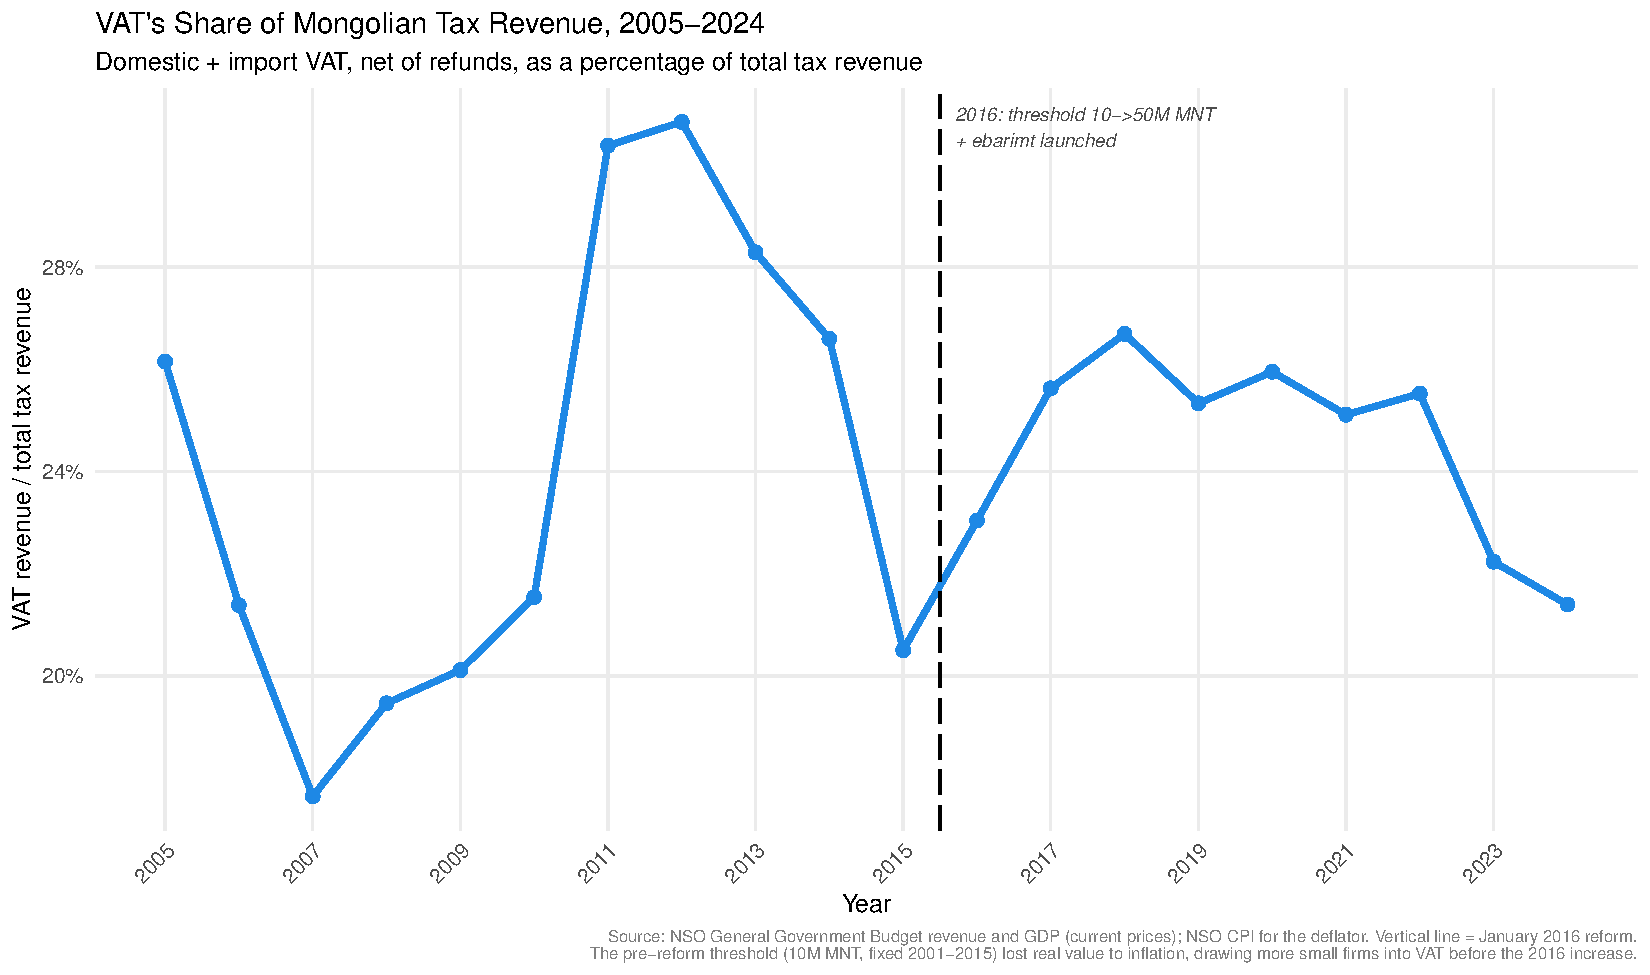
\includegraphics[width=\textwidth]{Figures/fig_vat_tax_share.pdf}
  \vspace{0.5em}
  \\ \footnotesize
  \begin{minipage}{0.92\textwidth}
  \small\textit{Notes:} Value-added tax (domestic plus import VAT, net of
  refunds) as a percentage of total tax revenue. The vertical dashed line
  marks the January 2016 reform (registration threshold 10M~$\rightarrow$~50M
  MNT and the launch of ebarimt). \textit{Source:} NSO General Government
  Budget revenue \parencite{nso_government_budget}.
  \end{minipage}
\end{figure}

In January 2016, the revised VAT Law enacted two reforms at once. First, the registration threshold rose fivefold to 50 million MNT (about 23,000 USD), reducing compliance obligations for smaller firms and letting the authority concentrate enforcement on larger businesses. In real terms the change was closer to a restoration than a fivefold increase, since indexation alone would have carried the 2001 cutoff to 35 to 40 million MNT. Second, the government launched ebarimt, an electronic receipt system aimed at strengthening compliance in retail transactions by drawing consumers into enforcement. A further amendment, adopted in June 2026 and effective from January 2027, raises the threshold again to 400 million MNT (about USD 113,000) \parencite{vatamendment2026}; it postdates the sample and does not affect the estimates.

Ebarimt gives consumers a financial reason to request and register receipts. Those who upload receipts through the mobile application receive a rebate equal to 20 percent of the VAT paid and enter monthly lottery draws with prizes up to 20 million MNT (about 9,300 USD) \parencite{mta_publication_2023}.\footnote{If no top-prize winner is identified, the prize rolls over, up to a maximum jackpot of 500 million MNT (about 232,000 USD).} Consumers can also report firms that refuse to issue receipts directly through the application. On the firm side, businesses must install point-of-sale systems linked to the ebarimt network \parencite{nyamdavaa2023does}; once a receipt is issued, the transaction is transmitted to the tax authority regardless of whether the consumer later registers it. Reporting thus occurs at the point of sale rather than through subsequent consumer action, and non-compliant firms face administrative penalties.

The reform therefore altered monitoring of B2C transactions specifically, while B2B transactions already left an invoice trail (Chapter~\ref{ch:lit_review}). This asymmetry is the basis for using B2B sectors as the comparison group throughout the analysis, and Section~\ref{sec:theoretical_framework} formalises it.

\section{Theoretical Framework}
\label{sec:theoretical_framework}

This section formalises how a discrete tax notch induces revenue compression and how the asymmetric enforcement shock of Section~\ref{sec:institutional} shifts that compression differentially across sectors.

Consider a continuum of firms indexed by productivity $n \in [n_L, n_H]$. Each firm chooses reported annual revenue $z$ to maximise utility subject to the VAT threshold $z^*_t$, which equals $z_1^* = 10{,}000{,}000$ MNT (about 4,700 USD) before the reform (2014--2015) and $z_2^* = 50{,}000{,}000$ MNT (about 23,000 USD) after (2016--2023). In both regimes the schedule introduces a discrete notch:
\begin{equation}
T(z;\, z^*_t) =
\begin{cases}
0       & \text{if } z < z^*_t \\
\tau z  & \text{if } z \geq z^*_t
\end{cases}
\end{equation}
where $\tau = 0.10$ is the statutory rate. A firm crossing $z^*_t$ faces a discrete liability jump of $\Delta T = \tau z^*_t$, creating an incentive to report just below the threshold \parencite{kleven2013using,kleven2016bunching}. Because $\Delta T$ scales with $z^*_t$, this mechanical incentive is five times larger after 2016 ($\Delta T_2 = 5{,}000{,}000$ MNT (about 2,300 USD)) than before ($\Delta T_1 = 1{,}000{,}000$ MNT (about 470 USD)).

For B2C sales, where consumers cannot claim downstream VAT credits, the VAT effectively acts as a tax on gross revenue, making the registration decision particularly relevant for consumer-facing firms \parencite{liu2021vat}.\footnote{\textcite{naritomi2019consumers} models tax as proportional to gross reported revenue and notes the logic extends to VAT when reported expenses do not fully offset reported revenue; \textcite{harju2019compliance} model the notch as a levy on value added, with the incentive scaling in the value-added share.} For B2B sectors the incentive is weaker, since registered buyers reclaim the seller's output VAT. This is the identification lever: B2B sectors supply the counterfactual trend rather than the object of inference.

A proportional notch generates a dominated region just above the threshold \parencite{kleven2013using, kleven2016bunching}, though heterogeneous input shares blur its upper edge \parencite{harju2019compliance, liu2021vat}. Recovering the structural elasticity $\epsilon$ from the marginal-buncher condition requires parametric assumptions that cannot be credibly met with binned, sector-level data \parencite{blomquist2021bunching}. I therefore do not recover $\epsilon$ and treat the reduced-form bunching ratio as the primary estimand:
\begin{equation}
    \hat{b}_{st}
    \;=\;
    \frac{\hat{B}_{st}}{\overline{\hat{N}}_{R_t}}
    \label{eq:b_hat_theory}
\end{equation}
where $\hat{B}_{st}$ is the excess firm count in the bunching window and $\overline{\hat N}_{R_t}$ the average counterfactual count over it; normalising by the local counterfactual height removes the mechanical thinning of the firm distribution at higher revenue.

Where transactions are hard to verify and cash is common, firms reach the threshold by under-reporting rather than by cutting real output. Following \textcite{allingham1972income}, let $y$ be true revenue and $p(s,t) \in (0,1)$ the sector-time audit probability. A firm with $y > z^*_t$ under-reports to $z \approx z^*_t$ and bunches when the expected profit from doing so exceeds honest compliance:
\begin{equation}
\underbrace{y}_{\text{Untaxed at }z^*_t}
\;-\; p(s,t)\bigl[(\tau+\theta)(y-z^*_t)\bigr]
\;-\; c(y-z^*_t)
\;>\;
\underbrace{y(1-\tau)}_{\text{Honest compliance}}
\label{eq:bunching_condition}
\end{equation}
where $\theta > 0$ is a proportional penalty on concealed revenue and $c(\cdot)$ a strictly convex friction cost with $c(0)=0$.\footnote{If detected with probability $p(s,t)$, the authority recovers true revenue $y$ and assesses the omitted VAT $\tau(y-z^*_t)$ plus a fine $\theta(y-z^*_t)$, following Allingham--Sandmo (1972).} The condition defines a productivity threshold below which firms manipulate, and the excess mass widens as the evasion zone widens. Differentiating the boundary condition gives the two comparative statics that drive the empirical work:
\begin{equation}
    \frac{\partial\hat{b}_{st}}{\partial z^*_t} > 0
    \quad \text{and} \quad
    \frac{\partial\hat{b}_{st}}{\partial p(s,t)} < 0 .
    \label{eq:comparative_static}
\end{equation}
A higher threshold raises bunching by enlarging the untaxed allowance and the liability jump; a higher detection probability lowers it by raising the expected cost of concealment. Nothing in the empirical design depends on the level of $\epsilon$; the model is used only for the signs in equation~\eqref{eq:comparative_static} and the three predictions that follow.

The 2016 reform moves both arguments at once. The threshold rises from 10M to 50M for all sectors, pushing $\hat{b}$ up everywhere. Ebarimt adds an enforcement shock $\Delta p > 0$ that reaches only consumer-facing sectors through POS-linked third-party reporting, so that $p(\text{B2C}, t \geq 2016) = p(\text{B2C}, t < 2016) + \Delta p$ while $p(\text{B2B}, t \geq 2016) \approx p(\text{B2B}, t < 2016)$.\footnote{E-receipts transmit automatically once the POS terminal is online, with at most three working days' delay \parencite{nyamdavaa2023does}. Rollout was gradual, about 51 percent of retailers enrolled by 2016 and 56 percent by 2018, so $\Delta p$ is an average shock across the treated sector, not a uniform jump.} Combined with the pre-reform ordering $p(\text{B2C}, t<2016) \ll p(\text{B2B}, t)$, equation~\eqref{eq:comparative_static} yields three predictions:
\begin{enumerate}
    \item \textit{Pre-reform gap.} Weaker baseline B2C enforcement implies higher baseline bunching in B2C than B2B sectors at the 10M threshold.

    \item \textit{No secular B2B trend.} Facing no consumer-side shock, B2B excess mass should show no systematic post-reform decline, tracking the macro trajectory and the larger threshold and so providing the counterfactual for the pure threshold shift.\footnote{This is partially violated if ebarimt raised B2B compliance through invoice-matching pressure \parencite{nyamdavaa2023does}; Section~\ref{sec:event} addresses this by excluding Wholesale Trade from the control group.}

    \item \textit{Negative DiD estimand.} Because $\Delta p$ offsets the threshold-induced rise more in B2C than B2B sectors,
    \begin{equation}
    \beta = \bigl(\hat{b}_{\text{B2C, Post}} - \hat{b}_{\text{B2C, Pre}}\bigr)
          - \bigl(\hat{b}_{\text{B2B, Post}} - \hat{b}_{\text{B2B, Pre}}\bigr) < 0 .
    \end{equation}
\end{enumerate}


\section{Data}
\label{subsec:descriptive}

I use administrative Corporate Income Tax (CIT) data from the Mongolian Tax Authority. Although the notches govern VAT registration, the CIT registry is well suited to bunching estimation because all incorporated entities must file income tax returns regardless of VAT status. The resulting revenue distribution therefore spans both sides of the threshold and avoids the survival selection inherent in VAT-only registries.

To protect confidentiality while preserving behavioral variation near the notches, the microdata are aggregated into a balanced panel of binned revenue frequencies. Gross annual revenues are sorted into uniform 1,000,000 MNT bins (about USD 470) from 0 to 400,000,000 MNT (about USD 186,000), yielding 400 bins per cross-section. The panel covers four sectors over 2014–2023, producing 40 sector-year cells. Firms are classified according to their primary economic activity under the National Classification of Types of Economic Activity. The four sectors are defined at the division level: retail trade (Division 47) and food and beverage service activities (Division 56) form the B2C group, while wholesale trade (Division 46) and manufacturing (Section C) form the B2B group.

The aggregated format rules out firm-level covariates and individual-level robustness checks common in microdata studies \parencite{harju2019compliance, liu2021vat, muthitacharoen2021vat}, but it suits the estimator, which operates directly on bin frequency counts \parencite{kleven2016bunching}, and the 400 bins per cell leave ample room to fit flexible polynomial counterfactuals.

The sample is divided by exposure to final consumers: the B2C treatment group is retail trade and food services, the B2B control group wholesale trade and manufacturing, for the reasons set out in Section~\ref{sec:theoretical_framework}. Any spillover of ebarimt to B2B suppliers would make the control partially treated; Section~\ref{sec:event} examines this.

\begin{table}[H]
\centering
\caption{\textbf{Aggregate Firm Distribution
         by Sector Group and Policy Regime}}
\label{tab:descriptive_stats}
\begin{threeparttable}
\setlength{\tabcolsep}{0pt}
\small
\begin{tabular*}{\linewidth}{l@{\extracolsep{\fill}}rrrr}
\toprule
& \multicolumn{2}{c}{\textit{Pre-Reform (2014--2015)}}
& \multicolumn{2}{c}{\textit{Post-Reform (2016--2023)}} \\
\cmidrule(lr){2-3}\cmidrule(lr){4-5}
Sector & \multicolumn{1}{c}{Mean Firms\tnote{a}}
& \multicolumn{1}{c}{Annual Total\tnote{b}}
& \multicolumn{1}{c}{Mean Firms\tnote{a}}
& \multicolumn{1}{c}{Annual Total\tnote{b}} \\
\midrule
\multicolumn{5}{l}{\textit{B2C Treatment Group}} \\[2pt]
\quad Food service         & 5.3 & 1,178 & 4.3 & 1,231 \\
\quad Retail               & 20.1 & 7,228 & 20.0 & 7,890 \\
[6pt]
\multicolumn{5}{l}{\textit{B2B Control Group}} \\[2pt]
\quad Manufacturing        & 8.9 & 3,015 & 9.3 & 3,393 \\
\quad Wholesale            & 19.2 & 7,519 & 23.9 & 9,564 \\
\bottomrule
\end{tabular*}
\begin{tablenotes}[para,flushleft]\footnotesize
\small\textit{Notes:}
\item[a] Average annual firms per active revenue bin across 400 bins (0--400M MNT).
\item[b] Mean annual firm count, excluding firms that filed a nil (``X'') return reporting no revenue.
\textit{Source:} MTA CIT registry.
\end{tablenotes}
\end{threeparttable}
\end{table}

Table~\ref{tab:descriptive_stats} shows that before the reform, retail and wholesale were comparable in size, averaging 7,228 and 7,519 firms per year, respectively, which supports wholesale as a comparison group. The largest post-reform change occurs in wholesale, where firms per bin increase by 24.5 percent, from 19.2 to 23.9. This pattern is consistent with the upstream spillover documented by \textcite{nyamdavaa2023does}: greater visibility of retail sales may have increased pressure on suppliers to report accurately. Food services, by contrast, decline modestly from 5.3 to 4.3 firms per bin, which more likely reflects redistribution of firms after the fivefold threshold increase than a real contraction of the sector. The implications for the estimated treatment effect are examined in Sections~\ref{sec:did} and~\ref{sec:event}.

The density discontinuity at the threshold is large (Appendix Table~\ref{tab:app_density_ratios}). In 2014 the bin just below $z^*_1 = 10{,}000{,}000$ MNT (about 4,700 USD) holds 1,105 retail firms against 98 just above, an 11.3:1 ratio. The B2B ratios are far lower (4.7:1 wholesale; 5.6:1 manufacturing), direct descriptive evidence of the B2C--B2B contrast and a first indication consistent with Prediction~1. By 2017 the B2C ratios compress (retail 3.3:1; food services 3.2:1) while the B2B ratios fall more modestly (wholesale 2.8:1; manufacturing 1.9:1). Figure~\ref{fig:raw_dist} shows the pattern.

\begin{figure}[H]
    \centering
    \caption{\textbf{Raw Revenue Distributions by Sector and Policy Era}}
    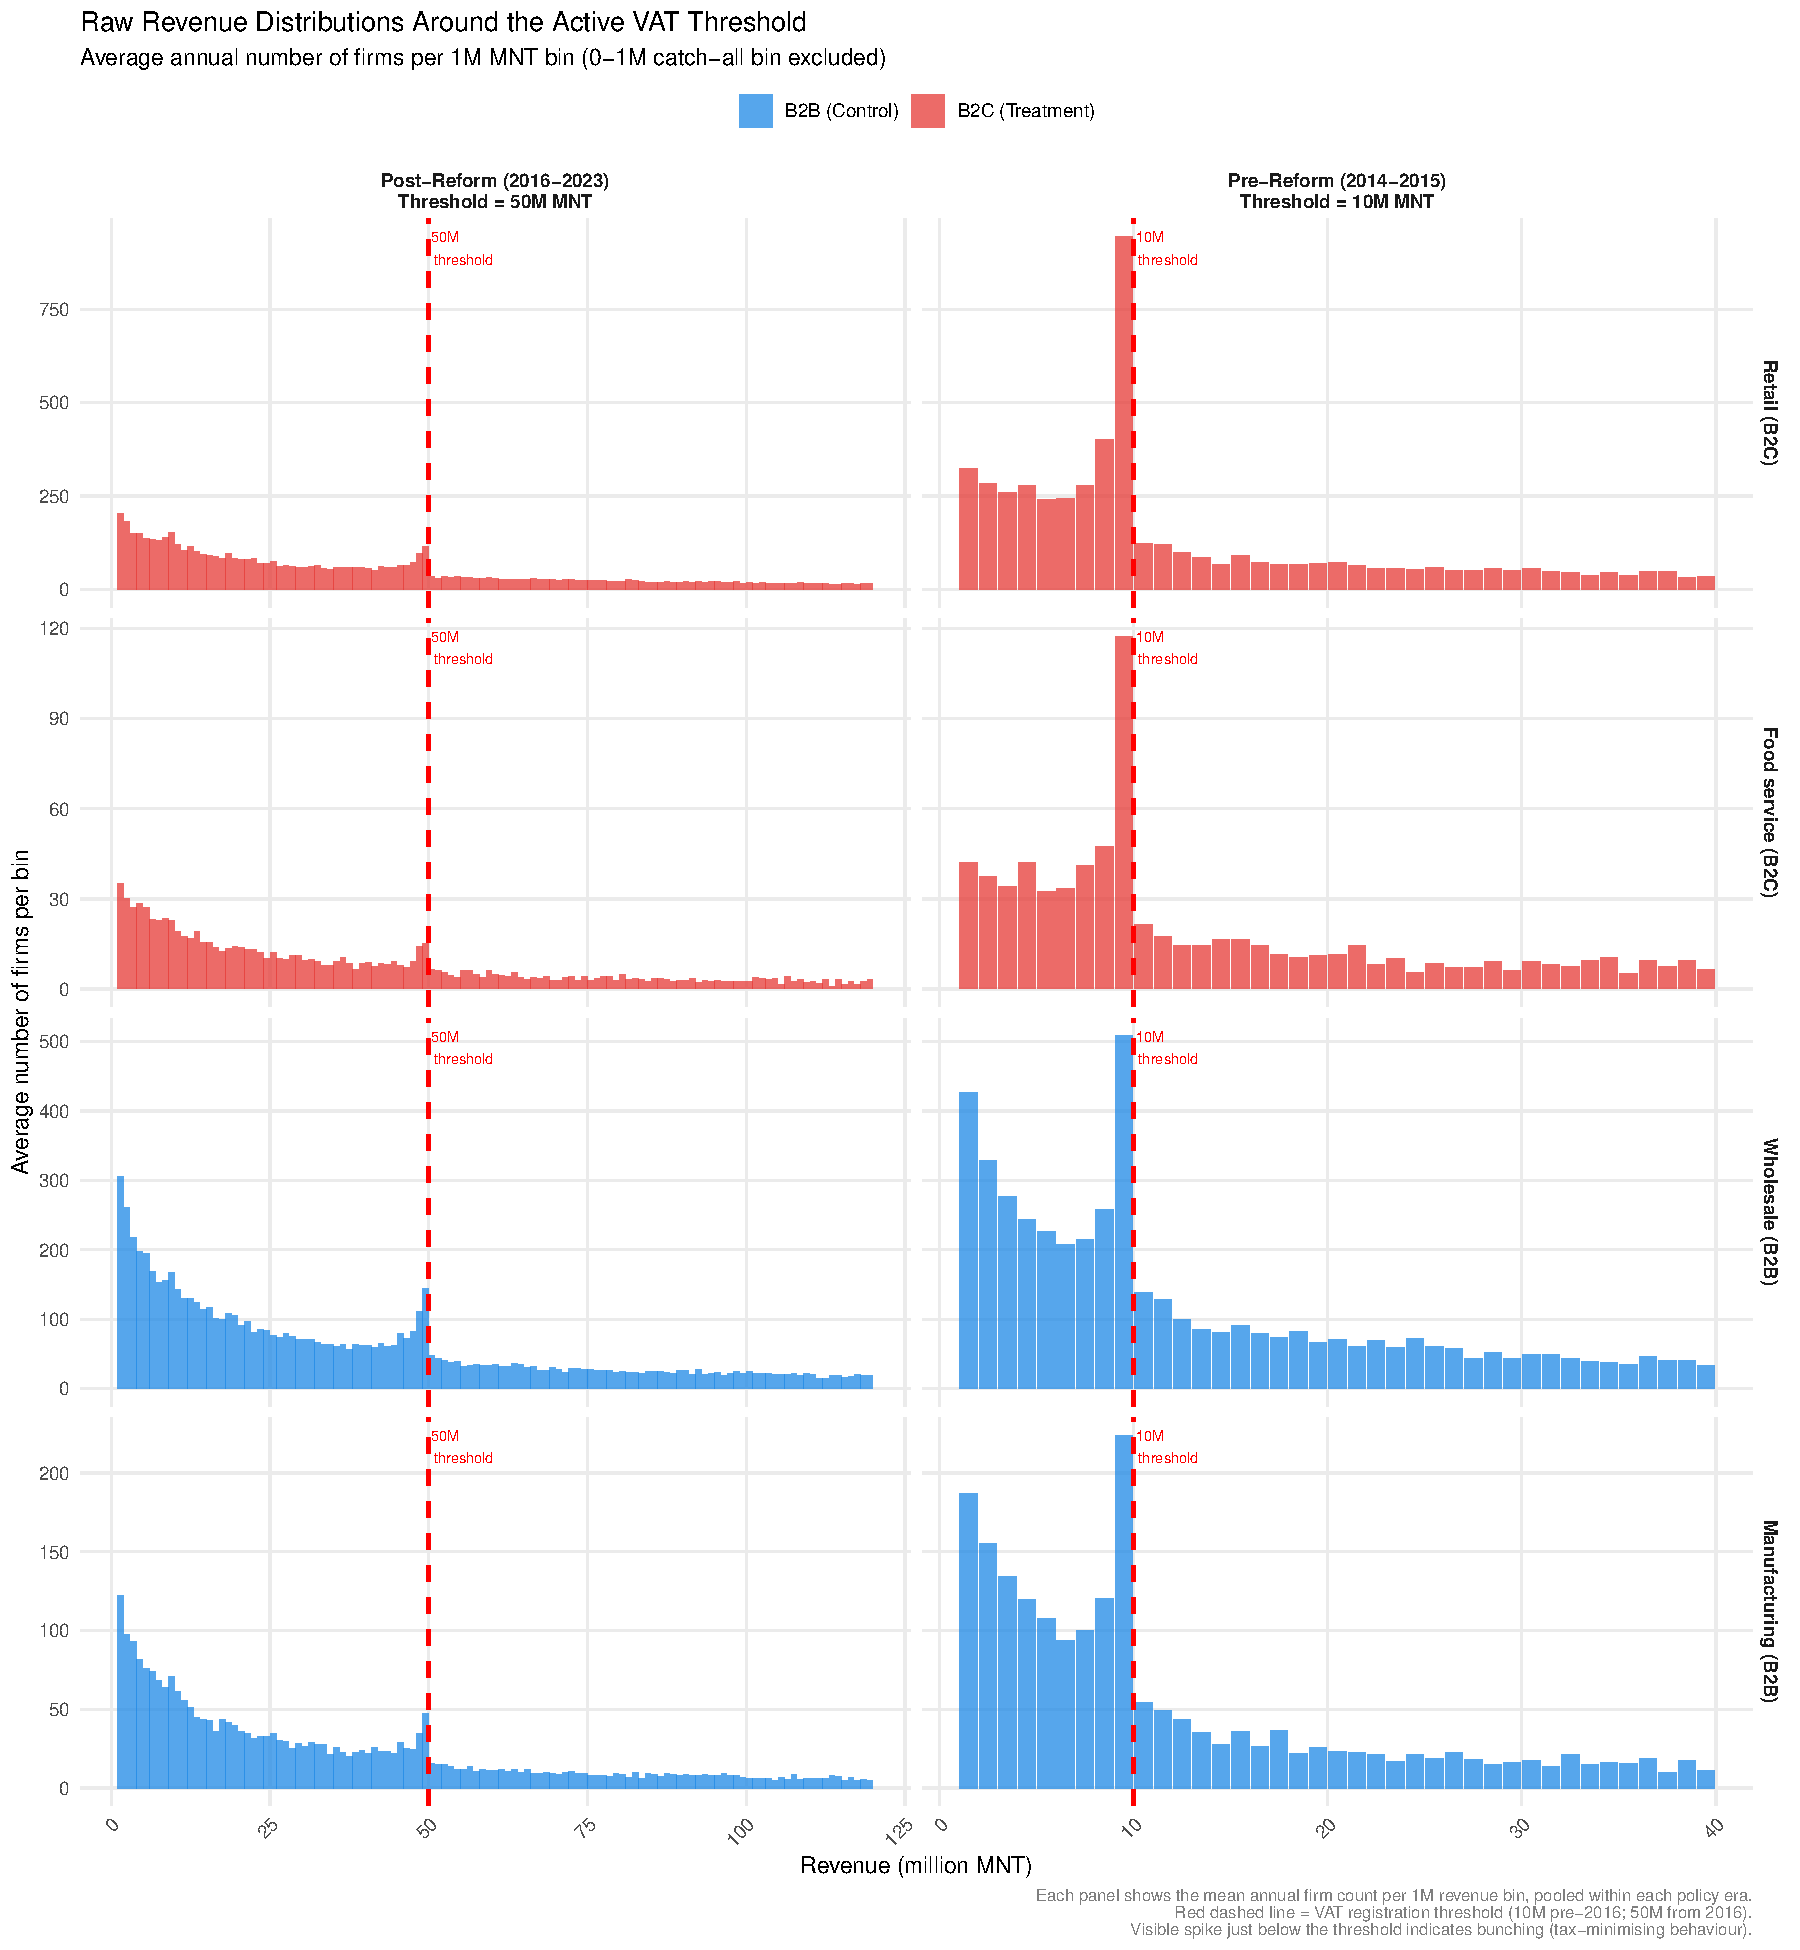
\includegraphics[width=\textwidth]{Figures/fig_desc_distributions.pdf}
    \label{fig:raw_dist}
    \small\textit{Notes:} Mean annual firms per 1 million MNT revenue bin by policy period. The [0,1M) MNT bin is excluded. Red dashed line marks the VAT threshold.
  \textit{Source:} MTA CIT registry.
\end{figure}

To protect parallel trends, the estimation samples vary in their treatment of the pandemic years, when containment policy hit the B2C and B2B groups asymmetrically. I define three nested samples:
\begin{enumerate}
    \item \textbf{Main (preferred):} 36 cells, 2014--2019 and 2021--2023, omitting 2020.
    \item \textbf{Robustness Sample A:} 32 cells, 2014--2019 and 2022--2023, omitting 2020 and 2021.
    \item \textbf{Full Sample:} all 40 cells, 2014--2023, retained as a conservative benchmark.
\end{enumerate}
The 2020 exclusion reflects Mongolia's zero-COVID measures, which closed in-person retail and food service (B2C) while freight exemptions kept wholesale and manufacturing (B2B) operating; the further 2021 exclusion in Sample~A reflects extended Ulaanbaatar lockdowns. Reporting all three samples shows how far the estimate moves with the pandemic years, which Section~\ref{sec:event} quantifies.

\section{Estimation Method}
\label{sec:estimation_method}

Estimation proceeds in two steps. First, for each sector-year I recover a normalised bunching ratio $\hat{b}_{st}$ using the polynomial counterfactual method of \textcite{chetty2011adjustment}, adapted to the notch setting following \textcite{kleven2013using}, \textcite{harju2019compliance}, and \textcite{liu2021vat}. Second, I use the recovered $\hat{b}_{st}$ as the outcome in a difference-in-differences design comparing B2C and B2B sectors around 2016.

\paragraph{The bunching estimate.} Let $N_{jst}$ be the firm count in bin $j$, sector $s$, year $t$, with midpoint $z_j$, and let
\begin{equation}
z^*_t =
\begin{cases}
10{,}000{,}000 \text{ MNT} & t \in \{2014, 2015\} \\
50{,}000{,}000 \text{ MNT} & t \in \{2016, \dots, 2023\}.
\end{cases}
\end{equation}
The smooth counterfactual $\hat{N}_{jst}$ is recovered in three steps.

\paragraph{Step 1: counterfactual fit.}
A polynomial centred at the threshold is fitted to the observed distribution, with dummies absorbing the bins inside an exclusion window $W_t$,
\begin{equation}
N_{jst} = \sum_{k=0}^{p}\gamma_k\bigl(z_j - z^*_t\bigr)^{k}
         + \sum_{l \in W_t}\nu_l\,\mathbb{I}(j = l)
         + u_{jst},
\label{eq:poly_fit}
\end{equation}
with $p = 5$ pre-reform and $p = 7$ post-reform. The counterfactual is the polynomial prediction with the window dummies omitted, $\hat{N}_{jst} = \sum_{k=0}^{p}\hat{\gamma}_k(z_j - z^*_t)^{k}$, floored at zero. Since the dominated region scales with the threshold at a fixed rate \parencite{kleven2013using}, a window fixed in absolute MNT would be too narrow post-reform, so the windows scale with $z^*_t$:
\begin{equation}
W_t =
\begin{cases}
[\,z^*_1 - 2\text{M},\; z^*_1 + 10\text{M}\,) = [8\text{M},\, 20\text{M}) & t \in \{2014, 2015\} \\[4pt]
[\,z^*_2 - 2\text{M},\; z^*_2 + 30\text{M}\,) = [48\text{M},\, 80\text{M}) & t \in \{2016,\dots,2023\}.
\end{cases}
\label{eq:window}
\end{equation}
The lower edge sits 2M below the threshold in both regimes, capturing the spike just below $z^*_t$ without reaching the rising shoulder of the small-firm density (Figure~\ref{fig:raw_dist}); the upper edge is the maximum extent of the Step~2 search. Sensitivity to the window appears in Appendix Table~\ref{tab:app_excl_lo}.

\paragraph{Step 2: upper bound.}
The upper bound $z^U_t$ cannot be read directly from the data, since missing mass above a notch is diffuse. Following \textcite{kleven2013using}, it is pinned down by setting missing mass equal to bunching mass,
\begin{equation}
\hat{M}_{st} = \hat{B}_{st},
\qquad
\hat{M}_{st} = \sum_{j \in [z^*_t, z^U_t]}(\hat{N}_{jst} - N_{jst}),
\label{eq:mass_conservation}
\end{equation}
raising $z^U_t$ from $z^*_t$ in 1M increments, re-estimating the counterfactual at each step until equation~\eqref{eq:mass_conservation} first holds, capped at the upper edge of $W_t$. Where the condition is met within the cap, it holds up to the 1M increment; in cells with no clean upper hole it has no interior solution, and $z^U_t$ is set to the cap and the cell flagged.

\paragraph{Step 3: bunching ratio.}
The bunching window is $R_t = [z^*_t - 2{,}000{,}000,\; z^*_t)$, narrower than $W_t$ by design: $W_t$ must reach far enough from the threshold to fit the counterfactual on unaffected bins, whereas bunching is a near-point mass in the bin just below $z^*_t$. Bins farther down carry near-zero excess mass, so widening $R_t$ would dilute $\hat{b}_{st}$; stability to alternative widths is confirmed in Appendix Table~\ref{tab:app_excl_lo}. The excess frequency is $\hat{B}_{st} = \sum_{j \in R_t}(N_{jst} - \hat{N}_{jst})$, and
\begin{equation}
\hat{b}_{st} = \frac{\hat{B}_{st}}{\overline{\hat{N}}_{R_t}},
\qquad
\overline{\hat{N}}_{R_t} = \frac{1}{|R_t|}\sum_{j \in R_t}\hat{N}_{jst}.
\label{eq:b_hat_emp}
\end{equation}
Standard errors for $\hat{b}_{st}$ come from a residual bootstrap with 500 replications within each cell \parencite{chetty2011adjustment}: I resample the residuals of equation~\eqref{eq:poly_fit}, regenerate bin counts, and re-estimate $\hat{b}_{st}$, holding $z^U_t$ fixed across replications. Because $\hat{b}_{st}$ is a reduced-form outcome rather than an input to a structural elasticity, I follow \textcite{liu2021vat} in not converting it to an elasticity: for a VAT notch, heterogeneous input costs prevent a cleanly defined dominated region above the threshold \parencite{harju2019compliance}, and the structural recovery that \textcite{harju2019compliance} undertake requires firm-level data on inputs and compliance costs that binned sector counts cannot supply.

\paragraph{The difference-in-differences estimate.}
The recovered ratios enter a two-step difference-in-differences design,
\begin{equation}
\hat{b}_{st} = \alpha + \beta\,(\mathrm{Post}_t \times \mathrm{Treated}_s)
             + \gamma_s + \delta_t + \eta_{st},
\label{eq:did}
\end{equation}
where $\mathrm{Post}_t = \mathbb{I}(t \geq 2016)$ and $\mathrm{Treated}_s = 1$ for the B2C sectors (retail and food service), $0$ for the B2B sectors (wholesale and manufacturing). Sector effects $\gamma_s$ absorb time-invariant industry differences; year effects $\delta_t$ absorb common shocks and the economy-wide level shift in $\hat{b}$ from the threshold increase. Because that increase applies to all sectors by statute, the differential B2C--B2B change in $\hat{b}_{st}$ is attributable to ebarimt to the extent that the threshold increase shifts both groups equally; under that common-threshold assumption, $\beta$ identifies the effect of consumer monitoring. This is the central identifying restriction of the analysis. Because no sector received the higher threshold without ebarimt, it cannot be tested directly; Section~\ref{sec:event} sets out the evidence that bears on it.\footnote{$\beta$ is not collinear with $\delta_t$: the year effects absorb the common annual level of $\hat{b}$ across both groups, while $\beta$ identifies only the treated-minus-control deviation.}

Two features of the design warrant comment. First, $\hat{b}_{st}$ enters the second stage as an estimated rather than observed outcome, a generated-dependent-variable structure. Second, the two-step approach is deliberate: \textcite{arkhangelsky2024causal} show that one-step alternatives, which pool the microdata and interact the policy directly, can be inconsistent because the treatment shifts the implicit estimation weights, whereas separating parameter estimation from policy evaluation avoids this. The within-cell residual bootstrap quantifies the first-stage error (Appendix Table~\ref{tab:app_bunching_main}); the second stage treats $\hat{b}_{st}$ as given and does not propagate that error jointly. The reported second-stage standard errors are therefore lower bounds, so the true $p$-values lie somewhat above those in Table~\ref{tab:did}, a simplification revisited in Chapter~\ref{ch:discussion}.

With only $G = 4$ clusters, asymptotic cluster-robust variance estimation over-rejects severely \parencite{cameron2008bootstrap, mackinnon2023cluster}. I therefore base inference on the restricted wild cluster bootstrap, imposing the null when generating bootstrap residuals \parencite{mackinnon2023cluster}, with Webb six-point weights: at $G = 4$, Rademacher weights admit only $2^4 = 16$ sign vectors and a minimum two-sided $p$-value of $0.125$, while Webb weights give $6^4 = 1{,}296$ distinct samples and finer resolution. I draw $B = 9{,}999$ replications. Inference with four clusters remains limited; Section~\ref{sec:did} sets out how the bootstrap $p$-value is read alongside the other evidence.

To assess parallel trends and trace timing, I estimate
\begin{equation}
\hat{b}_{st} = \alpha
             + \sum_{t \neq 2015}\beta_t
               \bigl(\mathbb{I}(\mathrm{year} = t) \times \mathrm{Treated}_s\bigr)
             + \gamma_s + \delta_t + \eta_{st}.
\label{eq:event_study}
\end{equation}
The baseline year is $t_0 = 2015$, the last pre-reform year, which predates any anticipatory response to the threshold change. Pre-2016 estimates test parallel trends; post-reform estimates trace whether the response is immediate or accumulates with ebarimt coverage.

I report the three samples of Section~\ref{subsec:descriptive}, together with Robustness Sample~B, which drops wholesale trade from the control group to address possible ebarimt spillovers through supply linkages. Section~\ref{sec:event} examines how far the estimate moves with the pandemic years and with the spillover concern.

% ==================================================
%  CHAPTER 4: ESTIMATION RESULTS AND EMPIRICAL ANALYSIS
% ==================================================

\chapter{Estimation Results and Empirical Analysis}
\label{ch:results}

The results proceed in three steps: the bunching estimates that motivate the causal analysis (Section~\ref{sec:bunching}), the difference-in-differences estimate and its inference (Section~\ref{sec:did}), and the dynamics and credibility checks (Section~\ref{sec:event}).


\section{Non-Parametric Bunching Estimates and Baseline
         Density Analysis}
\label{sec:bunching}

The polynomial counterfactual of Section~\ref{sec:estimation_method} is applied to each of the 36 sector-year cells in the main sample, yielding the normalised ratio $\hat{b}_{st}$ and its bootstrap standard error. Figures~\ref{fig:app_raw_2014} and~\ref{fig:app_raw_2017} show the full 2014 and 2017 distributions for all four sectors; the 2014 retail density drop across $z_1^*$ documented in Section~\ref{subsec:descriptive} is the most pronounced raw case. Table~\ref{tab:bunching} reports the group means, and sector-level estimates for all 36 cells appear in Appendix Table~\ref{tab:app_bunching_main}.

\begin{table}[H]
\centering
\caption{\textbf{Normalised Bunching Estimates: Group Means and
         Enforcement Gap (Main Sample, 2020 Excluded)}}
\label{tab:bunching}
\begin{threeparttable}
\setlength{\tabcolsep}{0pt}
\small
\begin{tabular*}{\linewidth}{l@{\extracolsep{\fill}}ccccccccc}
\toprule
Structural Metric & 2014 & 2015 & 2016 & 2017 & 2018 & 2019 & 2021 & 2022 & 2023 \\
\midrule
B2C mean & 4.156 & 3.230 & 2.185 & 1.667 & 1.837 & 2.392 & 1.026 & 3.009 & 1.644 \\
B2B mean & 2.660 & 1.844 & 1.471 & 2.340 & 2.841 & 2.000 & 1.330 & 2.056 & 2.570 \\
\midrule
Gap (B2C $-$ B2B) & $+$1.497 & $+$1.386 & $+$0.715 & $-$0.673 & $-$1.004 & $+$0.393 & $-$0.304 & $+$0.953 & $-$0.926 \\
\bottomrule
\end{tabular*}
\begin{tablenotes}[para,flushleft]\footnotesize
\item \textit{Notes:} Group means of $\hat{b}_{st}$ estimated via a degree 5 pre-reform, degree 7 post-reform counterfactual (excl.\ window $[z^*_t - 2M,\, z^*_t + 30M)$ post-reform). B2C = retail trade + food services; B2B = wholesale + manufacturing. 2020 excluded. \textit{Source:} Author's calculations based on MTA CIT registry data.
\end{tablenotes}
\end{threeparttable}
\end{table}

Before the reform, B2C sectors bunch far harder than B2B: a mean $\hat{b}$ of $3.693$ against $2.252$, a baseline gap of $1.441$ standardised units. This matches Prediction~1 and the breakdown of VAT self-enforcement at the final consumer stage \parencite{pomeranz2015no}. The gap is widest in 2014, when retail records $\hat{b} = 4.368$ (SE $0.263$) and food service $\hat{b} = 3.945$ (SE $0.430$; Table~\ref{tab:app_bunching_main}). Most pre-reform cells are flagged in Table~\ref{tab:app_bunching_main}: the diffuse upper hole characteristic of a VAT notch, where heterogeneous input shares blur the missing-mass region \parencite{harju2019compliance, liu2021vat}, leaves estimated missing mass short of bunching mass, so $z^U_t$ is capped at the window edge. This affects the upper-bound search rather than the sub-threshold excess that defines $\hat{b}_{st}$, and the raw density discontinuities in Table~\ref{tab:app_density_ratios} (11.3:1 in retail against 4.7:1 in wholesale, 2014) show the same B2C--B2B gap with no counterfactual at all.

After the reform the gap narrows and turns negative. It first does so in 2017 ($-0.673$), as B2C $\hat{b}$ falls below the B2B control, and reads $-0.926$ in 2023 (B2C $1.644$ against B2B $2.570$). The year-to-year path is not monotone, with a temporary 2022 B2C spike driven by an anomalous food service estimate, but the post-reform gap sits well below its pre-reform level. Relative to B2B controls, B2C threshold distortions fell far enough to close the pre-existing gap.

The B2B control shows no secular decline. Wholesale is almost flat from 2014 to 2022, between $1.90$ and $2.30$ in every year but 2021, before a single high reading of $3.006$ in 2023; manufacturing is noisier but returns to its pre-reform level by 2023. This is the pattern Prediction~2 requires of sectors outside consumer monitoring. Section~\ref{sec:event} returns to wholesale in the contamination check.

\begin{figure}[H]
    \centering
    \caption{\textbf{Normalised Bunching Ratio $\hat{b}_{st}$ by Sector,
         2014--2023}}
    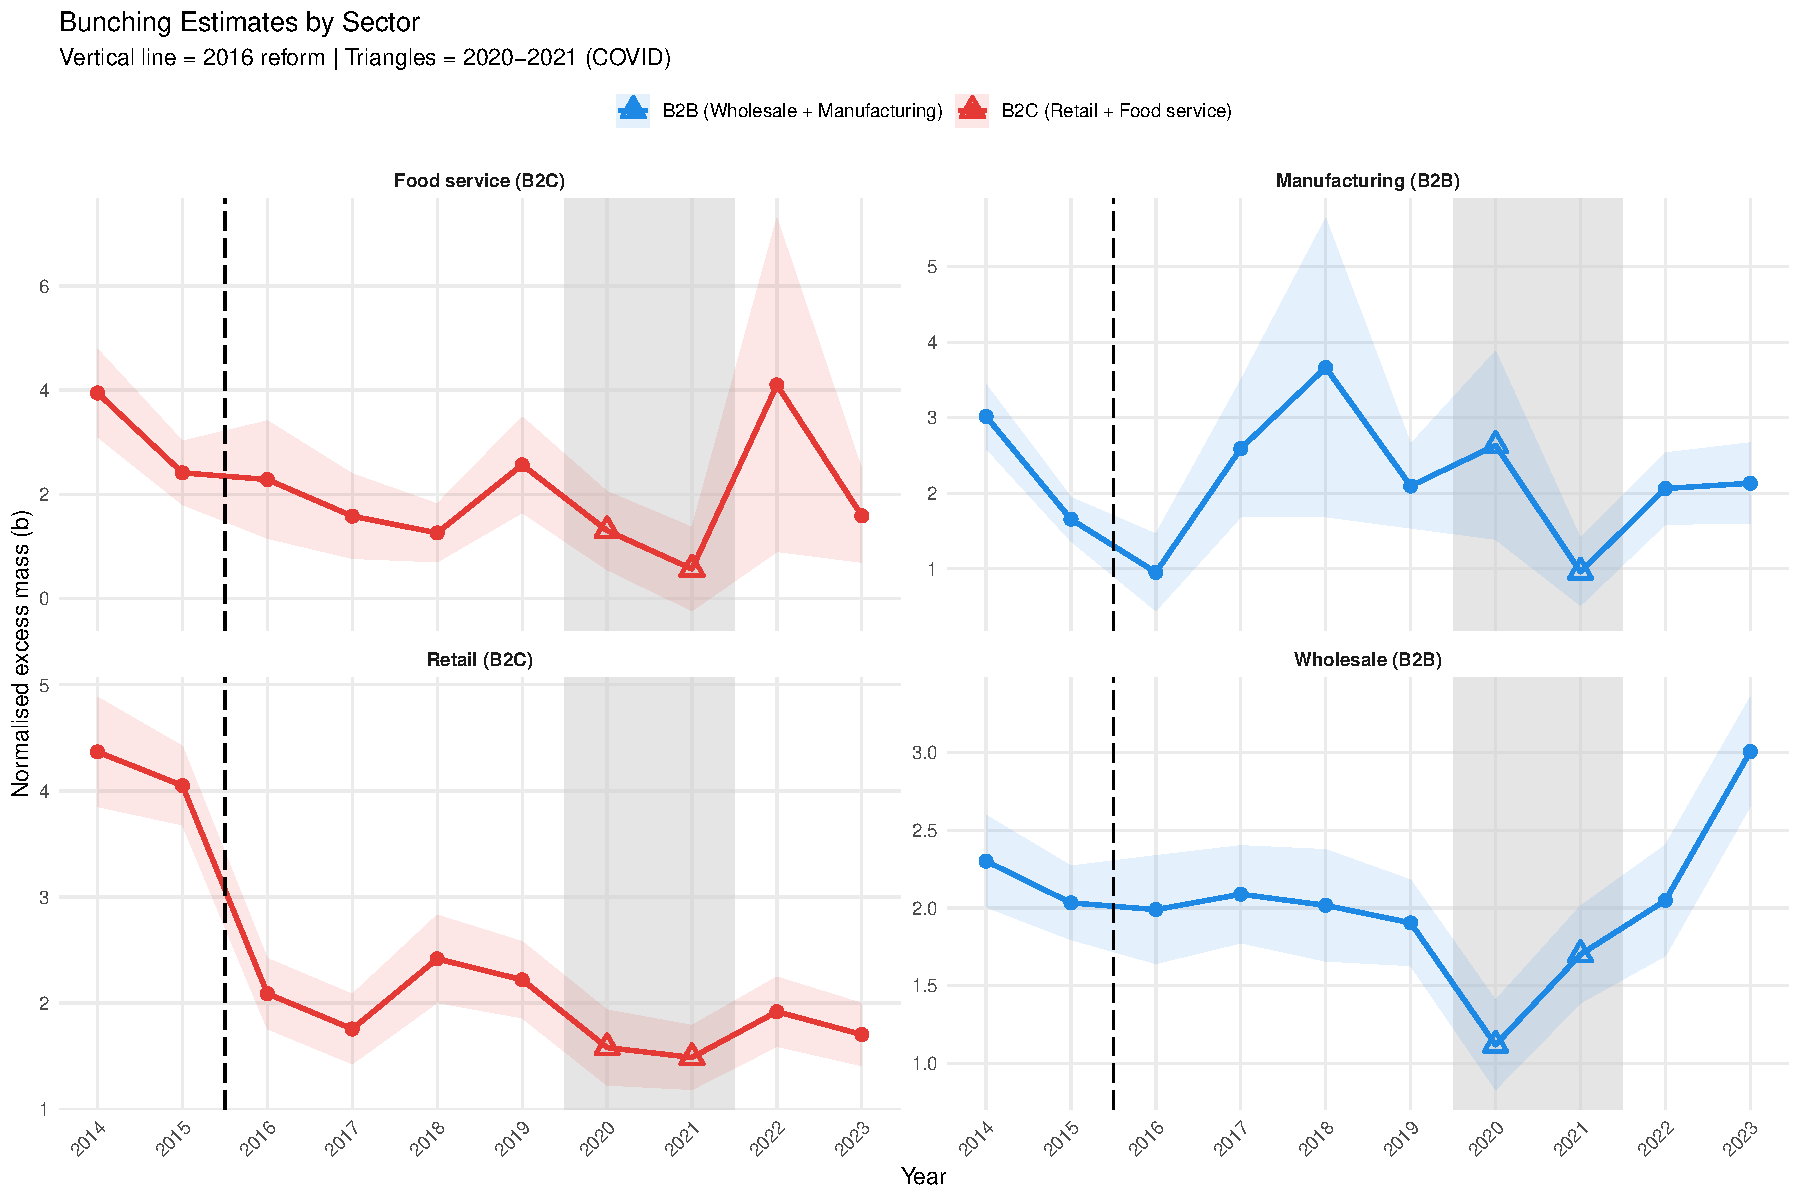
\includegraphics[width=\textwidth]{Figures/fig2_sector_bunching.pdf}
\label{fig:sector_bhat}
\small\textit{Notes:} Sector-specific $\hat{b}_{st}$ estimates with 95\% bootstrap confidence intervals (shaded). The dashed line marks the January 2016 VAT reform. Triangles indicate 2020 and 2021, the years affected by the COVID-19 pandemic.
 \textit{Source:} Author's calculations based on MTA CIT registry data.
\end{figure}

Figure~\ref{fig:sector_bhat} plots the four sectors separately, and the clearest contrast is between food service and manufacturing (sector-year values in Table~\ref{tab:app_bunching_main}). Food service shows the sharpest pre-reform decline of any sector, from $3.945$ in 2014 to $2.411$ in 2015, and sits below its 2015 level in every post-reform year except 2019 and the anomalous 2022 reading, reaching $0.564$ in 2021, implying little excess mass below the new 50M MNT threshold. This pattern is what the mechanism of Section~\ref{sec:theoretical_framework} would produce in the sector most exposed to foot traffic and receipt scanning: a rise in $p(\text{B2C}, t \geq 2016)$ removes the expected gain from evasion for all but the most productive firms, and the bunching mass collapses with it. The pattern echoes \textcite{naritomi2019consumers}, who finds the response largest among smaller firms and in sectors where firms face many different consumers, so that any one of them may blow the whistle. The 2022 food service reading ($\hat{b} = 4.099$) is an outlier from sparse near-threshold bins and an ill-conditioned counterfactual; it does not survive the polynomial-degree checks in Appendix Table~\ref{tab:app_robust_polynomial}.

Manufacturing, by contrast, is volatile but trendless: it swings from $0.952$ (2016) to $3.665$ (2018) on wide bootstrap intervals (SE $0.26$ and $1.01$), dips to $0.959$ in 2021, and recovers to $2.063$ (2022) and $2.133$ (2023), close to its pre-reform mean of $2.337$. The paths diverge in what matters. Food service declines before the reform and settles well below its pre-reform level, whereas manufacturing has no secular decline and returns to its pre-reform level by 2023. The 2021 dip is consistent with COVID-era supply disruption rather than a compliance shift, as Section~\ref{sec:event} examines directly. With no exposure to consumer monitoring, manufacturing bunching tracks the macroeconomy and the structure of the new notch, which is the comparison the design requires.

Figures~\ref{fig:app_cf_2015} and~\ref{fig:app_cf_2022} present the counterfactual overlays for retail and food service in 2015 and 2022, bracketing the reform. The fits track the observed density smoothly away from the exclusion window, and the predicted holes above the threshold match the missing mass implied by the notch, so the estimated excess mass is not an artefact of window selection. The overlays also fix the magnitude: in 2015 the retail bunching window holds an excess of roughly 768 firms ($\hat{b} = 4.05$) above the counterfactual; by 2022 that excess falls to about 100 firms ($\hat{b} = 1.92$). The raw count overstates the behavioural change, because fewer firms sit near the higher 50 million MNT threshold; the scale-free ratio falls by 53 percent, which is the relevant comparison. Food service moves the same way over most of the window, with $\hat{b}$ falling from $2.41$ in 2015 toward its floor by 2021 (the elevated 2022 reading is the artefact noted above and is set aside).


\section{Primary Difference-in-Differences Estimation Results}
\label{sec:did}

The sector-year ratios from Table~\ref{tab:bunching} enter the two-step DiD framework of Equation~\eqref{eq:did}. Figure~\ref{fig:did_bar} shows the $2\times2$ decomposition: mean $\hat{b}$ for the B2C and B2B groups across the pre- and post-reform periods.

\begin{figure}[H]
    \centering
    \caption{\textbf{2$\times$2 DiD: Mean Normalised Bunching Before and After the 2016 Reform}}
    \label{fig:did_bar}
    \vspace{4pt}

    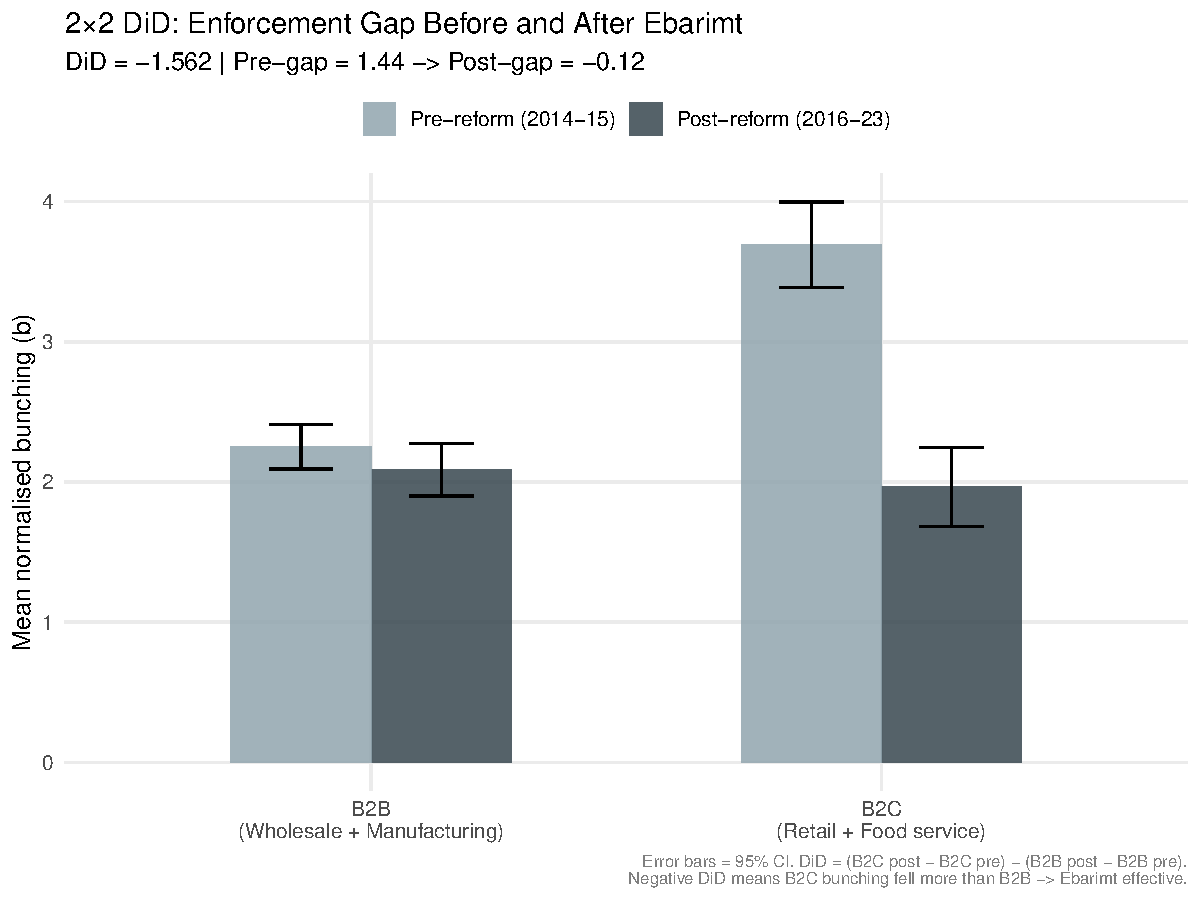
\includegraphics[width=0.72\textwidth]{Figures/fig4_did_bar.pdf}

    \vspace{6pt}
    \begin{flushleft}
    \small\textit{Notes:} Group means of $\hat{b}_{st}$ by treatment group and policy regime. Error bars denote 95\% confidence intervals. Pre-reform period: 2014--2015; post-reform period: 2016--2023, excluding 2020. The baseline DiD estimate ($\hat{\beta}=-1.562$) is from the Main specification (Table~\ref{tab:did}, column 1). \textit{Source:} Author's calculations based on MTA CIT registry data.
    \end{flushleft}
\end{figure}

The decomposition is direct (Table~\ref{tab:did}, column~1). B2C mean $\hat{b}$ falls from $3.693$ pre-reform to $1.966$ post-reform, a within-group decline of $1.727$ units, while the B2B control falls only from $2.252$ to $2.087$, a change of $-0.165$. Under parallel trends, the B2B trajectory supplies the counterfactual: the threshold shift alone would have reduced B2C bunching by about $0.165$ units, so the residual reduction attributable to the differential enforcement shock is $1.727 - 0.165 = 1.562 = -\hat{\beta}$. The regression confirms this:
\begin{equation}
\hat{\beta} = -1.562 .
\label{eq:did_result}
\end{equation}
This compresses the pre-reform enforcement gap from $+1.441$ to $-0.121$ standardised units, closing the original differential and turning its point estimate slightly negative. The reliable finding is convergence rather than reversal, since the post-reform gap is small relative to the year-to-year variation in Table~\ref{tab:bunching}; even so, convergence of this size is hard to explain without a change in how consumer-stage sales are verified. Figure~\ref{fig:enforcement_gap} traces this convergence over the full sample period.

\begin{figure}[H]
    \centering
    \caption{\textbf{B2C vs.\ B2B Normalised Bunching Over Time and the Convergence of the Enforcement Gap}}
    \label{fig:enforcement_gap}
    \vspace{4pt}

    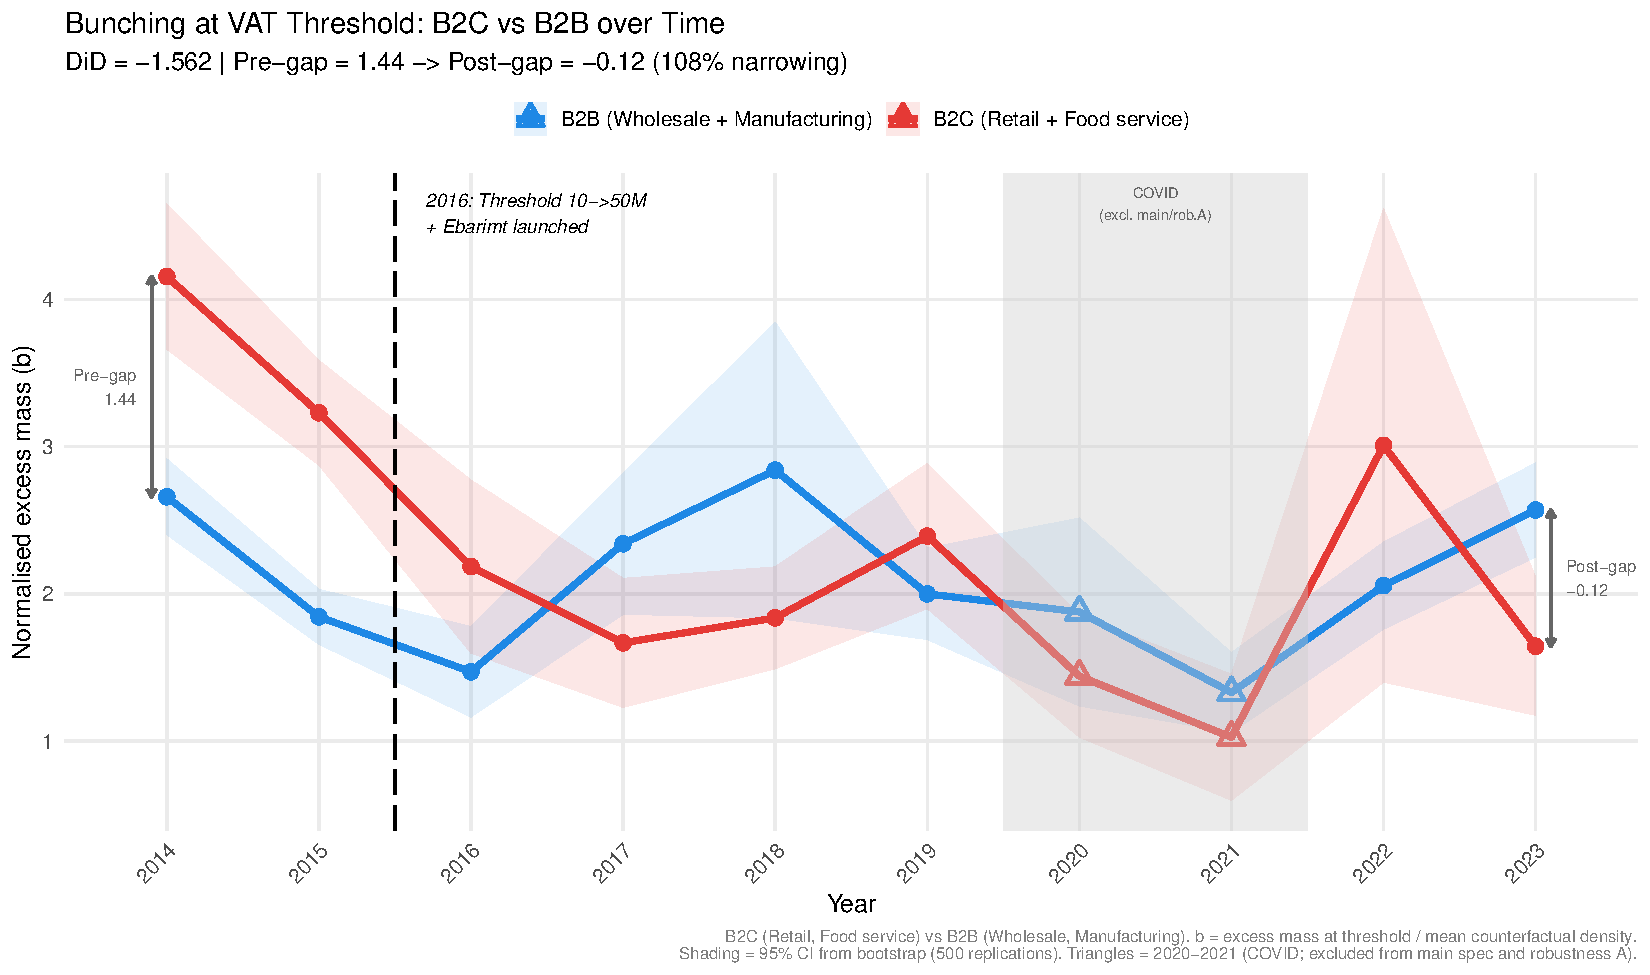
\includegraphics[width=\textwidth]{Figures/fig1_enforcement_gap_convergence.pdf}

    \vspace{6pt}
    \begin{flushleft}
    \small\textit{Notes:} Pooled B2C and B2B mean $\hat{b}_{st}$ series with 95\% bootstrap confidence intervals (shaded). The dashed line marks the January 2016 reform. The benchmark DiD estimate ($\hat{\beta}=-1.562$) implies a 108\% reduction in the initial B2C--B2B gap. Triangles indicate the COVID-19 years.
  \textit{Source:} Author's calculations based on MTA CIT registry data.
    \end{flushleft}
\end{figure}

% TABLE 4.2: DiD RESULTS
\begin{table}[H]
\centering
\caption{\textbf{Difference-in-Differences Estimation Results: Three Samples}}
\label{tab:did}
\begin{threeparttable}
\begin{tabular}{lccc}
\toprule
 & (1) Main & (2) Rob.\ A & (3) Full Sample \\
 & (2020 excl.) & (2020+21 excl.) & (all years) \\
\midrule
$\hat{\beta}$: Post $\times$ Treated
  & $-1.562^{*}$ & $-1.532^{*}$ & $-1.602^{*}$ \\
  & $(0.554)$ & $(0.633)$ & $(0.519)$ \\
Webb $p$-value & 0.066 & 0.079 & 0.060 \\
\addlinespace
Pre-reform B2C mean $(\bar{\hat{b}})$ & $3.693$ & $3.693$ & $3.693$ \\
Post-reform B2C mean $(\bar{\hat{b}})$ & $1.966$ & $2.122$ & $1.900$ \\
Pre-reform B2B mean $(\bar{\hat{b}})$ & $2.252$ & $2.252$ & $2.252$ \\
Post-reform B2B mean $(\bar{\hat{b}})$ & $2.087$ & $2.213$ & $2.060$ \\
\addlinespace
Pre-reform enforcement gap & $+1.441$ & $+1.441$ & $+1.441$ \\
Post-reform enforcement gap & $-0.121$ & $-0.090$ & $-0.160$ \\
Gap compression & 108\% & 106\% & 111\% \\
\midrule
Sector FE     & Yes & Yes & Yes \\
Year FE       & Yes & Yes & Yes \\
2020 excluded & Yes & Yes & No  \\
2021 excluded & No  & Yes & No  \\
$N$ (cells)   & 36  & 32  & 40  \\
\bottomrule
\end{tabular}
\begin{tablenotes}[para,flushleft]\footnotesize
\item \textit{Notes:} Dependent variable: normalised bunching ratio $\hat{b}_{st}$. CR1 cluster-robust standard errors (clustered by sector, $G=4$) in parentheses. Significance stars are based on Webb wild cluster bootstrap inference \parencite{webb2023reworking} with 6-point weights ($B=9{,}999$ replications): $^{*}p<0.10$, $^{**}p<0.05$, $^{***}p<0.01$. Exclusion window: $[z^*_t-2M,\; z^*_t+30M)$ post-reform.
 \textit{Source:} Author's calculations based on MTA CIT registry data.
\end{tablenotes}
\end{threeparttable}
\end{table}

The sign and magnitude of $\hat{\beta}$ match Prediction~3 (Section~\ref{sec:theoretical_framework}). In the model, ebarimt raises $p(\text{B2C}, t \geq 2016)$ by $\Delta p > 0$, tightening the evasion margin through $\partial\hat{b}_{st}/\partial p(s,t) < 0$ (Equation~\eqref{eq:comparative_static}).\footnote{The nominally fixed post-reform threshold $z_2^* = 50{,}000{,}000$ MNT (about 23,000 USD) loses real value as inflation erodes it over 2016--2023. This does not confound $\hat{\beta}$: symmetric inflation affects all sectors and is absorbed by the year fixed effects $\delta_t$, while $\hat{\beta}$ is identified solely from differential B2C--B2B movement within each calendar year.}

\paragraph{The threshold-expansion confound.}
The 2016 reform bundled the fivefold threshold expansion with the ebarimt launch, and the expansion could in principle drive the result on its own if B2C and B2B firms were distributed differently around the notch. Section~\ref{sec:event} takes this up in full, together with the firm-size composition around each threshold.

Inference uses the restricted Webb wild cluster bootstrap of Section~\ref{sec:estimation_method}, appropriate at $G = 4$ clusters. The Main coefficient $\hat{\beta} = -1.562$ has Webb $p = 0.066$; the Full sample gives $-1.602$ ($p = 0.060$) and Robustness~A $-1.532$ ($p = 0.079$). With four clusters the bootstrap cannot resolve finer significance, so the case rests on the stability of the point estimate, which moves only $0.07$ units across specifications, and on the event-study pattern below rather than on significance stars.


\section{Identification, Dynamics, and Robustness}
\label{sec:event}

A credible reading of $\hat{\beta}$ requires that it reflect consumer monitoring rather than the coincident threshold increase, divergent pre-trends, the treatment of pandemic years, or contamination of the control group. This section takes these in turn: it first sets out why the 2016 reform can be treated as exogenous to the differential B2C--B2B margin the design exploits, then uses the event study to test parallel trends and trace the post-reform path, varies the sample to gauge sensitivity to the COVID years, and narrows the control group to check for spillover.

\paragraph{Exogeneity of the reform.}
The design treats the January 2016 reform as exogenous to the differential B2C--B2B margin it exploits. Two features of the setting support that reading, and a third, compositional, threat is testable and is tested here.

The reform was not a response to sector-specific bunching. The threshold increase and the ebarimt launch were enacted together in the revised VAT Law, and I do not claim they are legislatively independent; both share a single origin. What identification requires is weaker: only that the reform did not target the differential margin the design uses. The threshold applies to every sector by the same statutory rule, and nothing in the law conditions the cutoff or the receipt system on a sector's prior evasion. The enforcement shock reaches consumer-facing firms not by legislative design but through the technology of the receipt: ebarimt binds where sales are made to final consumers who can be induced to demand receipts, and is close to inert where transactions are already invoiced between firms (Section~\ref{sec:theoretical_framework}).

The threshold increase itself is best read as a broad administrative adjustment rather than a consumer-enforcement measure, which is what allows the year fixed effects to absorb it. Indexing the 2001 cutoff to consumer prices implies a 2016 figure of 35 to 40 million MNT (Section~\ref{sec:institutional}), of the same order as the actual 50 million, so the increase largely restored the threshold's real value and eased filing for small firms, a motive common to B2C and B2B alike. Because that motive is sector-neutral, the year effects absorb it, and only the differential response is left for ebarimt to explain. The B2B path bears this out: B2B $\hat{b}$ is essentially flat across the two regimes ($2.252$ to $2.087$; Table~\ref{tab:did}), so for the same expansion to pull B2C down by $1.7$ units it would have to act in opposite directions on two groups facing an identical notch.

The residual threat is compositional rather than legislative, and the data speak to it directly. If B2C and B2B sectors differed systematically in firm-size distribution near the notch, the common threshold shift could move the two groups by different amounts even absent any enforcement change. The threshold-zone composition weighs against this: B2C and B2B firm counts sit near parity in fixed windows around both the old and the new notch before the reform (B2C/B2B ratios of $1.13$ at the old notch and $0.88$ at the new one in 2014), and both groups expand into the new threshold zone afterwards, B2B faster than B2C in line with its faster firm growth overall (the new-zone ratio falls from $0.88$ in 2014 to $0.59$ in 2023; Appendix Table~\ref{tab:app_zone_composition} and Figure~\ref{fig:ratio_threshold}, with the underlying distributions in Figures~\ref{fig:app_dist_pre} and~\ref{fig:app_dist_post}). Because $\hat{b}_{st}$ is normalised by the local counterfactual height, differences in counts do not enter the estimate. The one systematic post-reform shift runs with the mechanism rather than against it: the ratio at the old 10M notch falls from $1.09$ in 2015 to $0.61$ by 2023 as consumer-facing firms vacate that neighbourhood. What the binned data cannot rule out is a difference in the shape of the two distributions at the notch, a limit taken up in Chapter~\ref{ch:discussion}; on the evidence available, the size composition is close to symmetric. The event study adds a temporal check, developed next: a composition-driven artefact of the threshold move would appear at once in 2016, whereas the differential emerges only as ebarimt coverage spreads.

With 2015 as the omitted base, the single pre-reform coefficient $\hat{\beta}_{2014} = +0.110$ ($p = 0.913$) is the parallel-trends test, and it is indistinguishable from zero, so the data give no evidence against parallel trends. Table~\ref{tab:event_study} and Figure~\ref{fig:event_study} report the full sequence; Robustness~A yields identical coefficients for all non-pandemic years.

% TABLE 4.3: EVENT STUDY
\begin{table}[H]
\centering
\caption{\textbf{Event Study Coefficients: B2C Differential Bunching
         Relative to the 2015 Reference Baseline}}
\label{tab:event_study}
\begin{threeparttable}
\setlength{\tabcolsep}{0pt}
\small
\begin{tabular*}{\linewidth}{l@{\extracolsep{\fill}}cccccc}
\toprule
 & \multicolumn{2}{c}{Main Specification}
 & \multicolumn{2}{c}{Robustness A}
 & \multicolumn{2}{c}{Full Sample} \\
 & \multicolumn{2}{c}{(2020 Omitted)}
 & \multicolumn{2}{c}{(2020 \& 2021 Omitted)}
 & \multicolumn{2}{c}{(All Years)} \\
\cmidrule(lr){2-3} \cmidrule(lr){4-5} \cmidrule(lr){6-7}
Year & $\hat{\beta}_t$ & $p$-value & $\hat{\beta}_t$ & $p$-value & $\hat{\beta}_t$ & $p$-value \\
\midrule
\multicolumn{7}{l}{\textit{Pre-Reform Horizon}} \\[2pt]
2014 & $+$0.110 & 0.913 & $+$0.110 & 0.915 & $+$0.110 & 0.913 \\
2015 & \multicolumn{2}{c}{0.000\; (Baseline)} & \multicolumn{2}{c}{0.000\; (Baseline)} & \multicolumn{2}{c}{0.000\; (Baseline)} \\
\midrule
\multicolumn{7}{l}{\textit{Post-Reform Horizon}} \\[2pt]
2016 & $-$0.671 & 0.508 & $-$0.671 & 0.520 & $-$0.671 & 0.508 \\
2017 & $-2.059^{*}$ & 0.054 & $-2.059^{*}$ & 0.063 & $-2.059^{*}$ & 0.053 \\
2018 & $-2.390^{**}$ & 0.028 & $-2.390^{**}$ & 0.034 & $-2.390^{**}$ & 0.027 \\
2019 & $-$0.994 & 0.331 & $-$0.994 & 0.346 & $-$0.994 & 0.331 \\
2021 & $-$1.690 & 0.108 & \multicolumn{2}{c}{---} & $-$1.690 & 0.106 \\
2022 & $-$0.433 & 0.668 & $-$0.433 & 0.677 & $-$0.433 & 0.669 \\
2023 & $-2.312^{**}$ & 0.033 & $-2.312^{**}$ & 0.039 & $-2.312^{**}$ & 0.032 \\
\bottomrule
\end{tabular*}
\begin{tablenotes}[para,flushleft]\footnotesize
\item \textit{Notes:} Dynamic event-study coefficients ($\hat{\beta}_t$) relative to 2015. The reported $p$-values and significance stars are based on conventional OLS inference, uncorrected for the four-cluster structure, and describe the dynamic path rather than formal tests; formal inference relies on the Webb wild cluster bootstrap DiD estimates in Table~\ref{tab:did}. $^{*}p<0.10$, $^{**}p<0.05$, $^{***}p<0.01$.
\textit{Source:} Author's calculations based on MTA CIT registry data.
\end{tablenotes}
\end{threeparttable}
\end{table}

The effect builds gradually rather than appearing at the reform date. The 2016 coefficient is small ($-0.671$); divergence emerges in 2017 ($-2.059$) and grows through 2018 ($-2.390$). Most of the B2C decline itself is front-loaded (B2C mean $3.230$ in 2015, $2.185$ in 2016, $1.667$ in 2017; Table~\ref{tab:bunching}); the differential widens into 2018 partly because the B2B mean rises over the same years, so the gradual build describes the gap rather than B2C bunching alone. The path is not perfectly monotone, with the 2019 and 2022 coefficients pulling back toward zero, but it does not fade: the differential peaks in 2018 and the most recent estimate, $\hat{\beta}_{2023} = -2.312$, is essentially as large. A one-time 2016 compliance shock would have produced its full differential in 2016; the small 2016 coefficient is easier to reconcile with a platform that firms and consumers took up progressively (Section~\ref{sec:theoretical_framework}), a reading Chapter~\ref{ch:discussion} returns to. The coefficient $p$-values in Table~\ref{tab:event_study} are conventional OLS, uncorrected for the four-cluster structure, so I read them as describing the dynamic path and the parallel-trends check rather than as formal tests; formal inference is reserved for the pooled DiD in Table~\ref{tab:did}.

The post-reform path runs through the pandemic years, and the three samples of Section~\ref{subsec:descriptive} isolate how much the result depends on them. The 2020 B2C estimates reflect closed shops rather than a compliance response: retail $\hat{b}_{2020} = 1.581$ and food service $1.301$ both fall below their 2019 values ($2.220$ and $2.565$; Table~\ref{tab:app_covid}) in the year in-person retail and food service were shut. The 2020 event-study coefficient appears only in the full sample ($-1.822$, $p = 0.083$) and is dropped from the Main and Robustness~A specifications.

Manufacturing in 2021 is the key diagnostic. As a pure B2B sector with no ebarimt exposure, its bunching should follow macro conditions and threshold incentives, not consumer monitoring. Yet $\hat{b}_{2021} = 0.959$ is a 54\% drop from the 2019 level of $2.096$, with recovery to $2.063$ by 2022. A V-shaped trough in an untreated sector is consistent with an external disruption, although manufacturing also read $0.952$ in 2016 with no pandemic, so the series is noisy in both years and the event-study coefficient $\hat{\beta}_{2021} = -1.690$ ($p = 0.108$) is best read as a transitional-year signal rather than a compliance shift. The Main specification keeps 2021; Robustness~A drops it.

\begin{figure}[H]
    \centering
    \caption{\textbf{Event Study: B2C Differential Bunching Trajectories Across Alternative Sample Definitions}}
    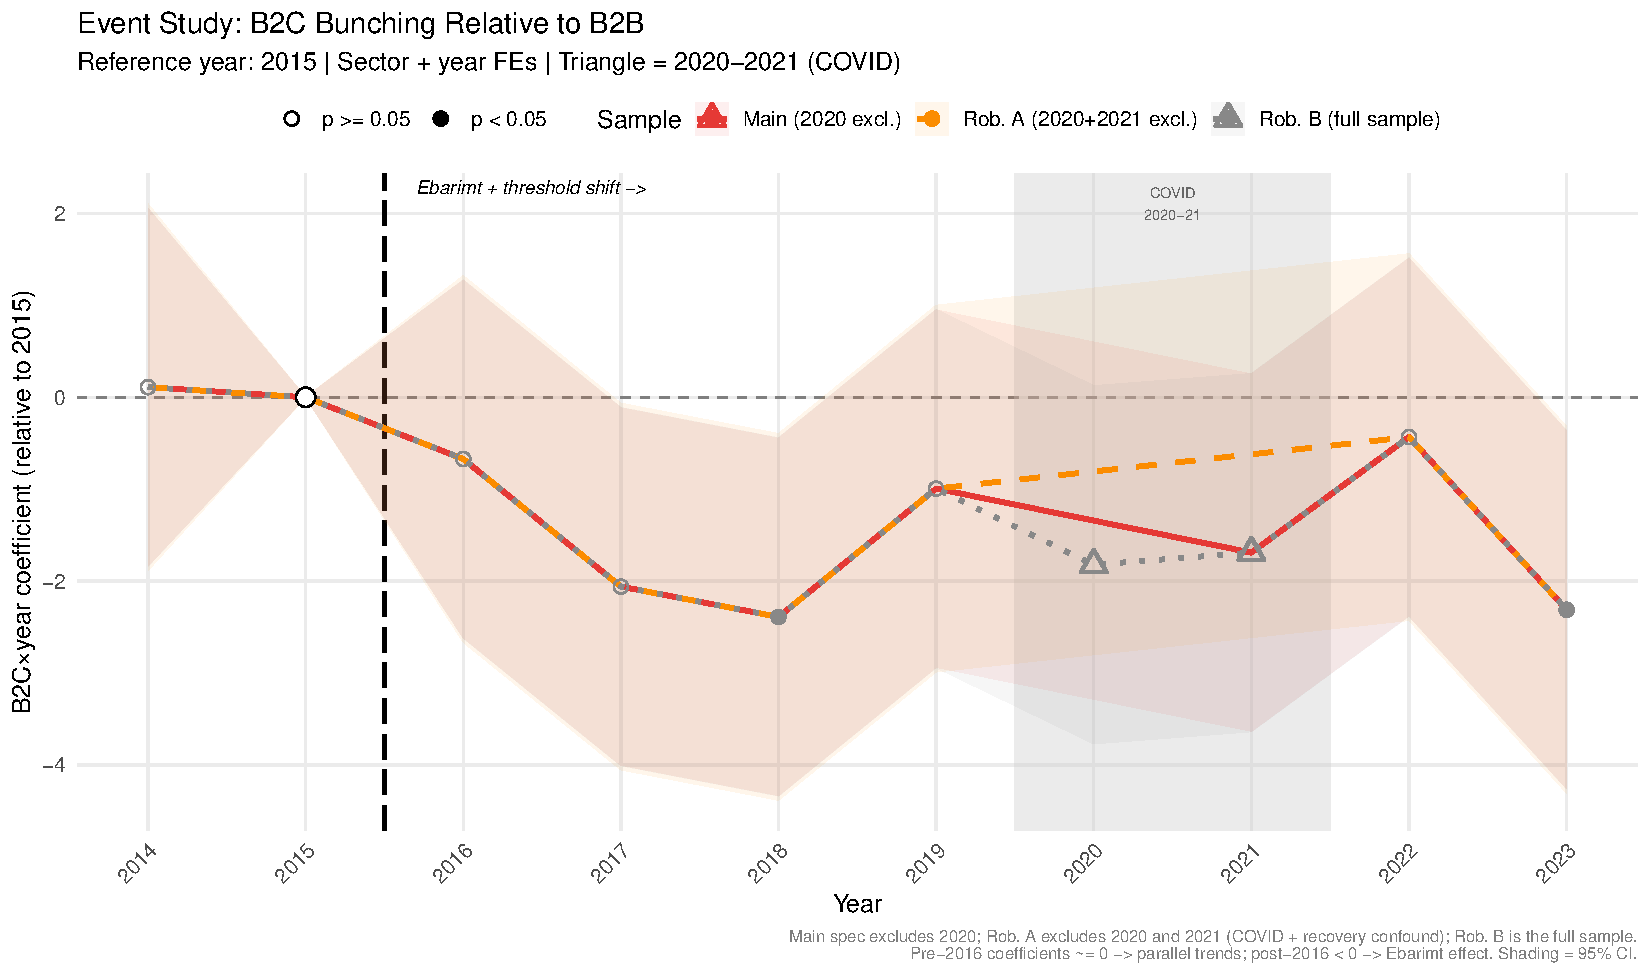
\includegraphics[width=\textwidth]{Figures/fig3_event_study.pdf}
\label{fig:event_study}
\small\textit{Notes:} Event-study coefficients ($\hat{\beta}_t$) with 95\% confidence intervals. Filled markers denote conventional OLS significance at the 5\% level, open markers its absence; see the notes to Table~\ref{tab:event_study} on their interpretation. Triangles denote the COVID-19 years (2020--2021). The dashed line marks the January 2016 reform.
 \textit{Source:} Author's calculations based on MTA CIT registry data.
\end{figure}

Across the three samples the DiD coefficient is $\hat{\beta}_{\text{Main}} = -1.562$ ($N = 36$), $\hat{\beta}_{\text{Rob.\,A}} = -1.532$ ($N = 32$), and $\hat{\beta}_{\text{Full}} = -1.602$ ($N = 40$), a range of $0.070$ units, under 5\% around the central estimate. The Full sample is marginally the most negative and Robustness~A the least; dropping 2021 removes a transitional year in which COVID disruption depressed manufacturing $\hat{b}$, and the resulting movement is small. The post-reform enforcement gap is closed in every sample ($-0.121$ Main, $-0.090$ Robustness~A, $-0.160$ Full). The Robustness~A event study (Figure~\ref{fig:event_study}, dashed line) is nearly identical to the Main specification for all non-COVID years, with 2018 and 2023 again the coefficients furthest from zero ($\hat{\beta}_{2023} = -2.312$).

\paragraph{Control-group contamination.} \textcite{nyamdavaa2023does} documents that ebarimt compliance gains among downstream B2C retailers spill upstream into suppliers' reporting. If that spillover reached wholesale, the control would be partially treated, its $\hat{b}$ depressed, and $\hat{\beta}$ biased toward zero. The wholesale series shows no such depression: it is flat at about $2.0$ from 2014 through 2022 (pre-reform mean $2.167$, post-reform mean $2.108$; Table~\ref{tab:app_bunching_main}), with a single high reading of $3.006$ in 2023, which is what Prediction~2 expects of a sector outside consumer monitoring. Restricting the control to manufacturing, which has no direct link to retail chains, gives $\hat{\beta} = -1.457$ (HC2 SE $= 0.563$, $p < 0.05$, $N = 27$; Appendix Table~\ref{tab:app_robust_mfg}), slightly closer to zero because manufacturing $\hat{b}$ itself fell modestly across the reform ($2.337$ to $2.066$). The manufacturing-only estimate is therefore the more conservative of the two, and it moves the four-sector result by only $0.1$ units; the toward-zero bias remains a theoretical possibility rather than a feature visible in the data.


% ==========================================
% CHAPTER 5: POLICY IMPLICATIONS AND CONCLUSION
% ==========================================

\chapter{Discussion, Revenue Implications, Limitations, and Conclusion}
\label{ch:discussion}

The Mongolian evidence suggests that the B2C enforcement gap is not a fixed feature of the credit-invoice VAT. Because ebarimt verifies sales through consumers rather than auditors, verification scales with the spread of a consumer technology rather than with the size of the audit bureaucracy. The difference-in-differences results bear this out: the pre-reform B2C--B2B gap closes, and the event study shows the differential widening over several years rather than appearing at the reform date, which fits a process of gradual adoption (Section~\ref{sec:event}).

The sector pattern points the same way. The response was fastest in retail, where $\hat{b}$ fell by half in the first post-reform year and stayed there; food service, which had already been declining before the reform, took a noisier path to a lower floor. Both are sectors where sales are made face to face and receipts are issued at the counter. One reform in one economy cannot establish how far this generalises, but the direction is informative. Where sales are visible and the monitoring technology is easy to use, consumer-driven verification may be a low-cost complement to conventional audit capacity; Section~\ref{sec:revenue} draws out what this implies for the registration threshold.

\section{Implications for Tax Revenue}
\label{sec:revenue}

The bunching estimates describe the shape of the reported revenue distribution. The amount of revenue ebarimt raised, and the full welfare assessment that would set it against the program's costs, lie beyond this paper's scope. The clearest evidence on the revenue effect, however, comes from \textcite{nyamdavaa2023does}, who uses administrative CIT and VAT returns and finds that reported liabilities among monitored retailers rose by about 31 percent after the reform, with a further gain of roughly 15 percent among their upstream suppliers; the response is concentrated in VAT rather than income tax, which firms can offset by inflating reported costs. Those gains are intensive-margin responses by design: his samples are firms already filing returns, and the estimates survive when restricted to firms that were VAT-liable throughout, so the 2016 threshold shift does not drive them. Threshold bunching is the margin his design sets aside: firms that had held reported revenue below the cutoff and now register instead.

The two results therefore describe different margins of the same reform, and neither quantifies the other. The intensive-margin gains he documents are likely the larger share of revenue, since they apply to every monitored firm rather than only to those near the cutoff, but that ordering is an inference rather than a measured decomposition. The threshold and the monitoring technology still interact, though. \textcite{kanbur2014thresholds} show that the optimal threshold is higher where small firms have more room to slip out of the tax net, and ebarimt cuts into that room in exactly the consumer-facing sectors where it was largest. In June 2026 Parliament raised the registration threshold from 50 to 400 million MNT (about USD 113,000) with effect from January 2027 \parencite{vatamendment2026}. In the four sectors studied here, 13,474 firms reported revenue in that band in 2023, of which 5,676 were in retail and food service.\footnote{Author's calculation from the MTA CIT registry. The binned data stop at 400 million MNT, so these are counts of firms the higher threshold removes from the registration requirement, not shares of the registered population.} The eightfold increase will therefore exempt several thousand consumer-facing firms whose sales ebarimt has only recently made cheap to observe.

These gains come with real costs. A consumer-monitoring program needs spending on information technology, data management, and the consumer rewards themselves, which in Mongolia include a rebate of one-fifth of the VAT paid and monthly lottery prizes. \textcite{nyamdavaa2023does} calculates that the trade sector's VAT payments had to rise by about 30 percent to cover the rebate, prizes and administration, and that the retailer response alone roughly meets that bar, with the CIT and upstream gains putting the program clearly in surplus. That calculation counts only the state's outlays. Whether the programme also passes a welfare test is open. Answering it would need direct estimates of firm compliance costs and consumer adoption costs, which no study of ebarimt has produced; \textcite{nyamdavaa2023does} notes that such estimates do not exist and argues that firms' costs are at least partly reflected in the CIT liabilities he measures.

\section{Limitations}
\label{sec:limitations}

Several constraints bound these conclusions. The data are binned and aggregated, so they cannot track individual firms or separate the bunching response into real-output adjustment and strategic misreporting. Treatment is identified at the sector level: the estimates show how the bunching distribution shifted within B2C relative to B2B, not how firms differed within each group. The outcome itself is a normalised bunching ratio, which measures how far the distortion moved in standardised terms; the excess counts in Section~\ref{sec:bunching} give how many firms sit in the bunching window, not which firms moved.

Identification is limited in three ways. The threshold increase and the ebarimt launch took effect together in 2016 and are best treated as a single regime change; the design does not separate them by timing, and since the higher cutoff applied to both groups, only the residual cross-sector difference is attributed to consumer monitoring. Section~\ref{sec:event} sets out why the threshold move can be read as a sector-neutral adjustment absorbed by the year fixed effects, and why the compositional channel through which it could still bias the estimate does not appear in the threshold-zone data; but the common-threshold assumption, that the increase moved B2C and B2B bunching by the same amount, remains an assumption rather than a separately tested fact, because the binned data cannot compare the two groups' full revenue distributions near the notch. The parallel-trends test is also limited, because only one pre-reform coefficient is estimable; that coefficient, $\hat{\beta}_{2014} = +0.110$, is indistinguishable from zero, which is consistent with parallel trends but far from proof. And the control group is exposed to cross-sector spillovers: if ebarimt raised B2B supplier compliance through invoice-matching pressure \parencite{nyamdavaa2023does}, the control is partially treated and $\hat{\beta}$ understates the true effect. Restricting the control to manufacturing, which has no direct retail supply link, leaves the estimate negative and of similar magnitude (Section~\ref{sec:event}).

Inference is constrained in two further ways. With only four sector clusters, even the Webb wild cluster bootstrap yields $p$-values that are small-sample approximations, and the confidence intervals are wide: the results establish the direction and rough magnitude of the response rather than a tightly bounded coefficient (Section~\ref{sec:did}). The bunching ratios also enter the difference-in-differences as estimated rather than observed outcomes. The within-cell bootstrap captures their first-stage uncertainty, but a joint two-step treatment in the spirit of \textcite{arkhangelsky2024causal} is infeasible with four groups, so the reported standard errors are conditional on the first-stage estimates. Those first-stage errors are tight for wholesale and retail throughout, but wide for manufacturing in 2017--2018 (bootstrap SEs $0.46$ and $1.01$) and for food service in the early post-reform years, which cautions against over-reading any single coefficient.

These limits indicate the natural next steps. Firm-level panel data would follow individual firms across the threshold, separate real output responses from misreporting, and deliver the narrower intervals that sector aggregates cannot; regional variation in ebarimt's rollout would supply a second source of identification and test whether the response scales with local enforcement intensity. The contribution here should be read accordingly: not a final accounting of ebarimt's effect, but an identification of it within real data constraints, and a basis for the more granular work that richer data will allow.


\section{Conclusion}
\label{sec:conclusion}

Mongolia's 2016 reform paired a fivefold rise in the VAT registration threshold with ebarimt, a receipt system that enlists consumers in monitoring retail sales. Using binned tax-return data and a bunching estimator embedded in a difference-in-differences design, I find that threshold bunching fell substantially more in consumer-facing sectors than in the business-to-business sectors that ebarimt could not reach, closing a pre-reform enforcement gap of $1.4$ standardised units, with the differential widening over several years as the platform spread. The estimate is stable across samples and control-group definitions, though inference from four sector clusters is necessarily coarse. The result adds a threshold-response margin to the evidence that consumer-side reporting can repair the weakest link in the VAT chain, and it cautions against raising the registration cutoff in exactly the sectors where that repair has taken hold.


% ── START THE APPENDIX ──
\clearpage
\appendix
\chapter*{Appendix}
\addcontentsline{toc}{chapter}{Appendix}
\renewcommand{\thesection}{\Alph{section}}
\counterwithin{table}{section}
\counterwithin{figure}{section}

\section{Baseline Parameter Profiles and COVID-Year Estimations}
\label{sec:appendix_baseline_profiles}

This appendix collects the year-by-year estimates behind the main results: the raw sector-year distributions, the 2020 and 2021 (COVID) estimates, and the full 36-cell table of $\hat{b}_{st}$.
% ── APPENDIX FIGURE A.1 ──
\begin{figure}[H]
    \centering
    \caption{\textbf{Revenue Distributions at the VAT Threshold: 2014 (Pre-Reform)}}
    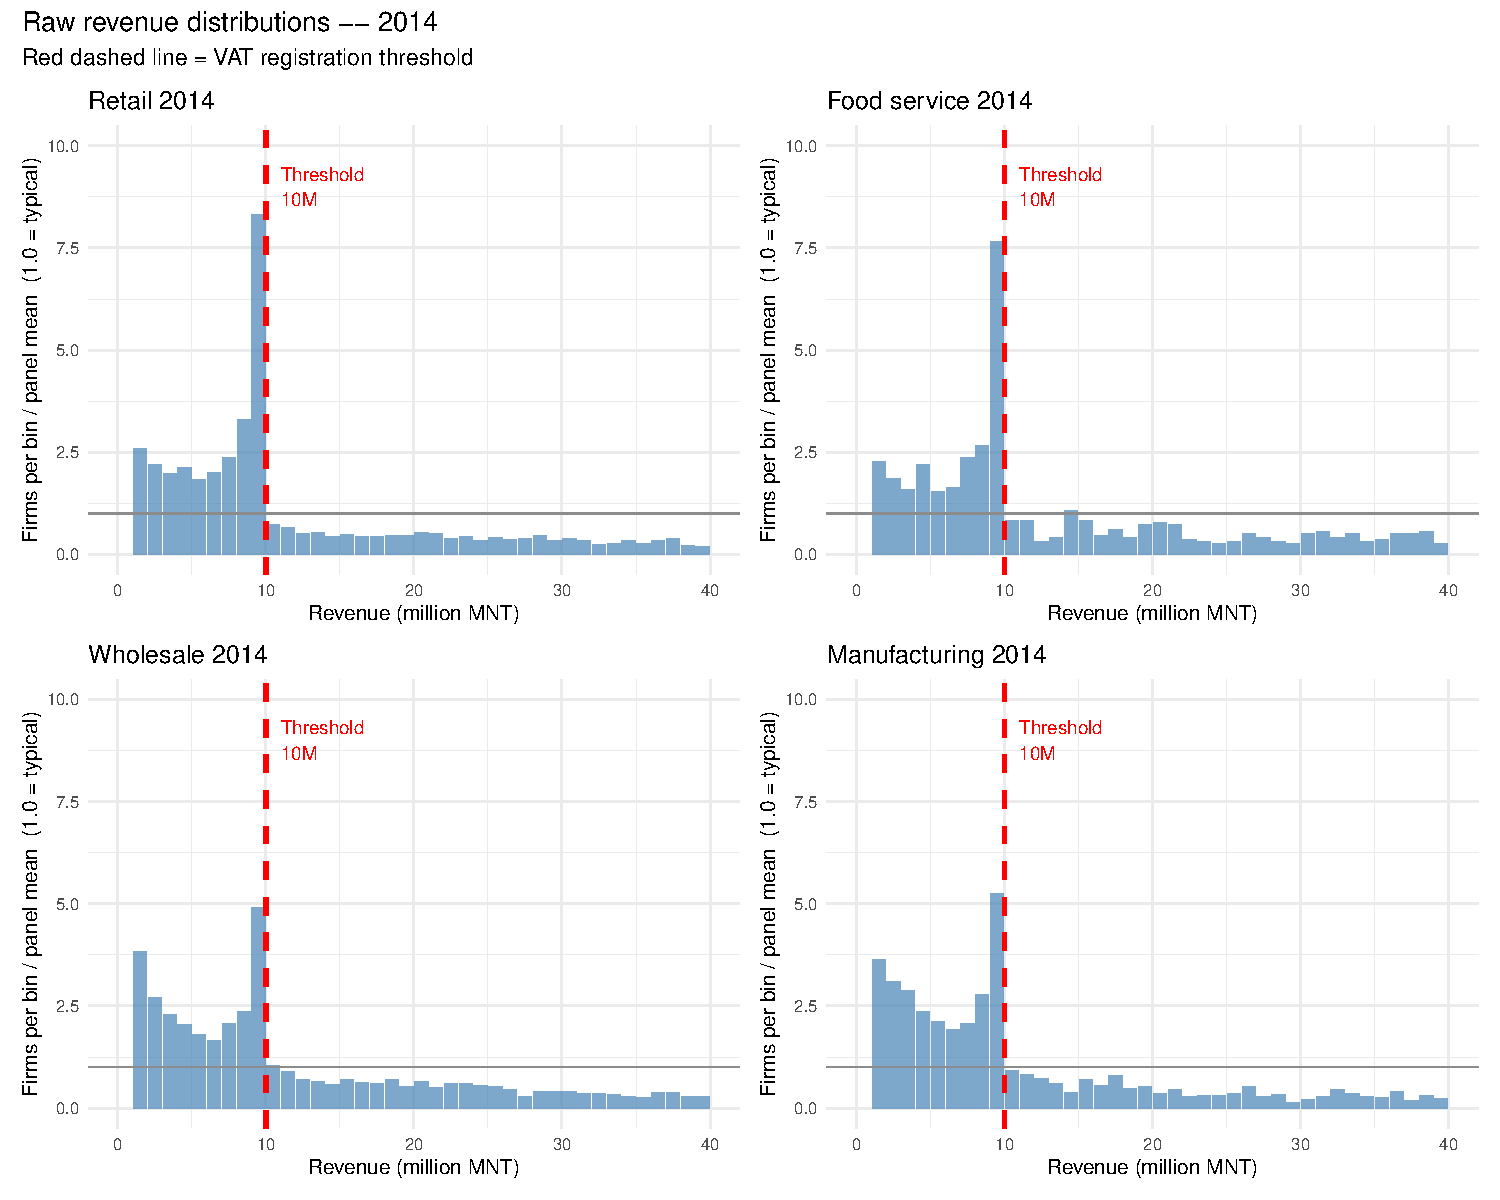
\includegraphics[width=\textwidth]{Figures/fig0_raw_distributions_2014.pdf}
    \label{fig:app_raw_2014}
    \small\textit{Source:} MTA CIT registry data.
\end{figure}

\begin{figure}[H]
    \centering
    \caption{\textbf{Revenue Distributions at the VAT Threshold: 2017 (Post-Reform)}}
    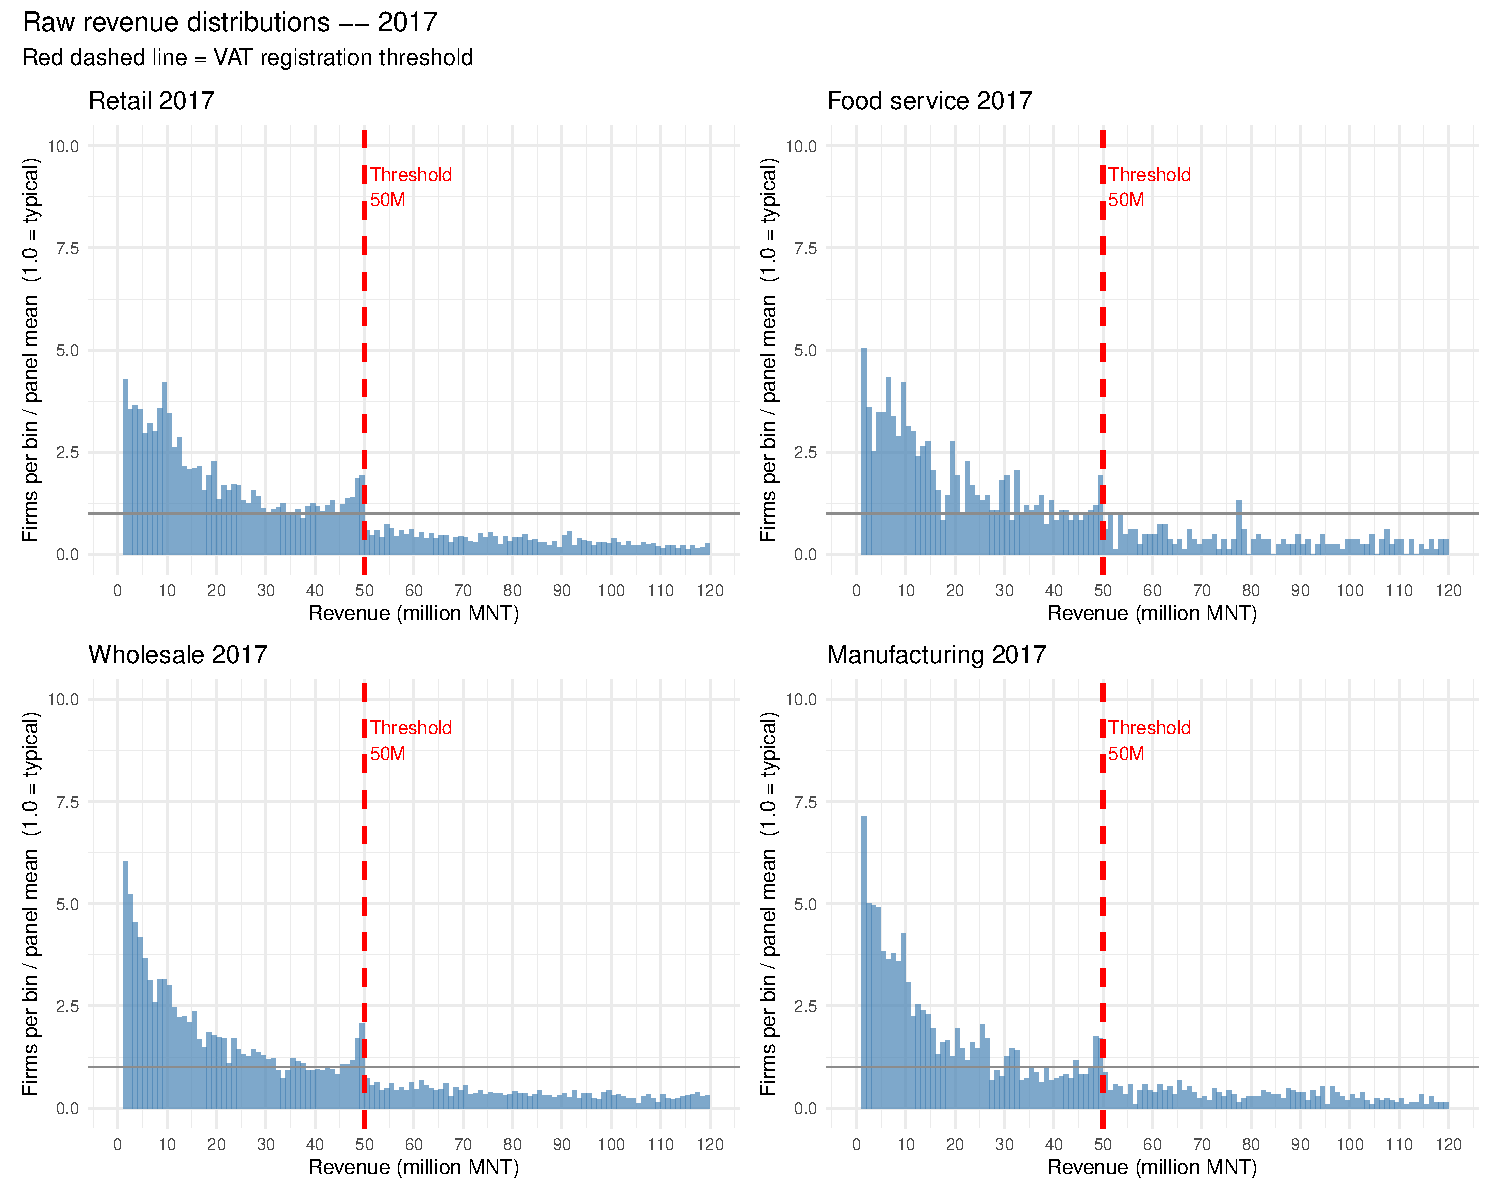
\includegraphics[width=\textwidth]{Figures/fig0_raw_distributions_2017.pdf}
    \label{fig:app_raw_2017}

    \footnotesize\textit{Notes:} Raw firm counts by 1M MNT revenue bins
    for each sector. The red dashed line is a VAT registration
    threshold at 50M MNT. The catch-all bin [0, 1{,}000{,}000) MNT is excluded.
     \textit{Source:} MTA CIT registry data.
\end{figure}

\vspace{1em}
% TABLE A.1 Density ratio at threshold
\begin{table}[H]
\centering
\caption{\textbf{Revenue Density Discontinuities at the Active Registration Threshold}}
\label{tab:app_density_ratios}
\begin{threeparttable}
\setlength{\tabcolsep}{0pt}
\small
\begin{tabular*}{\linewidth}{l@{\extracolsep{\fill}}cccccc}
\toprule
& \multicolumn{3}{c}{\textit{Pre-Reform: $z^*_1 = 10$M MNT (2014)}}
& \multicolumn{3}{c}{\textit{Post-Reform: $z^*_2 = 50$M MNT (2017)}} \\
\cmidrule(lr){2-4}\cmidrule(lr){5-7}
Sector & $N_{j^-}$\tnote{a} & $N_{j^+}$\tnote{b} & Ratio\tnote{c}
       & $N_{j^-}$\tnote{a} & $N_{j^+}$\tnote{b} & Ratio\tnote{c} \\
\midrule
\multicolumn{7}{l}{\textit{B2C Treatment Group}} \\[2pt]
\quad Retail Trade     & 1,105 & 98 & 11.3 & 101 & 31 & 3.3 \\
\quad Food Services    & 149 & 16 & 9.3 & 16 & 5 & 3.2 \\
[6pt]
\multicolumn{7}{l}{\textit{B2B Control Group}} \\[2pt]
\quad Wholesale Trade  & 582 & 123 & 4.7 & 118 & 42 & 2.8 \\
\quad Manufacturing    & 271 & 48 & 5.6 & 35 & 18 & 1.9 \\
\bottomrule
\end{tabular*}
\begin{tablenotes}[para,flushleft]\footnotesize
\item \textit{Source:} MTA CIT registry data.
\item[a] Firm count in the 1M MNT bin immediately below the threshold
  ($[z^*_t - 1\text{M},\, z^*_t)$).
\item[b] Firm count in the 1M MNT bin immediately above the threshold
  ($[z^*_t,\, z^*_t + 1\text{M})$).
\item[c] Density ratio $N_{j^-} / N_{j^+}$; values near 1 indicate
  no discontinuity.
\end{tablenotes}
\end{threeparttable}
\end{table}

\begin{figure}[H]
\centering
\caption{\textbf{B2C/B2B Firm Composition Near VAT Thresholds, 2014--2023}}
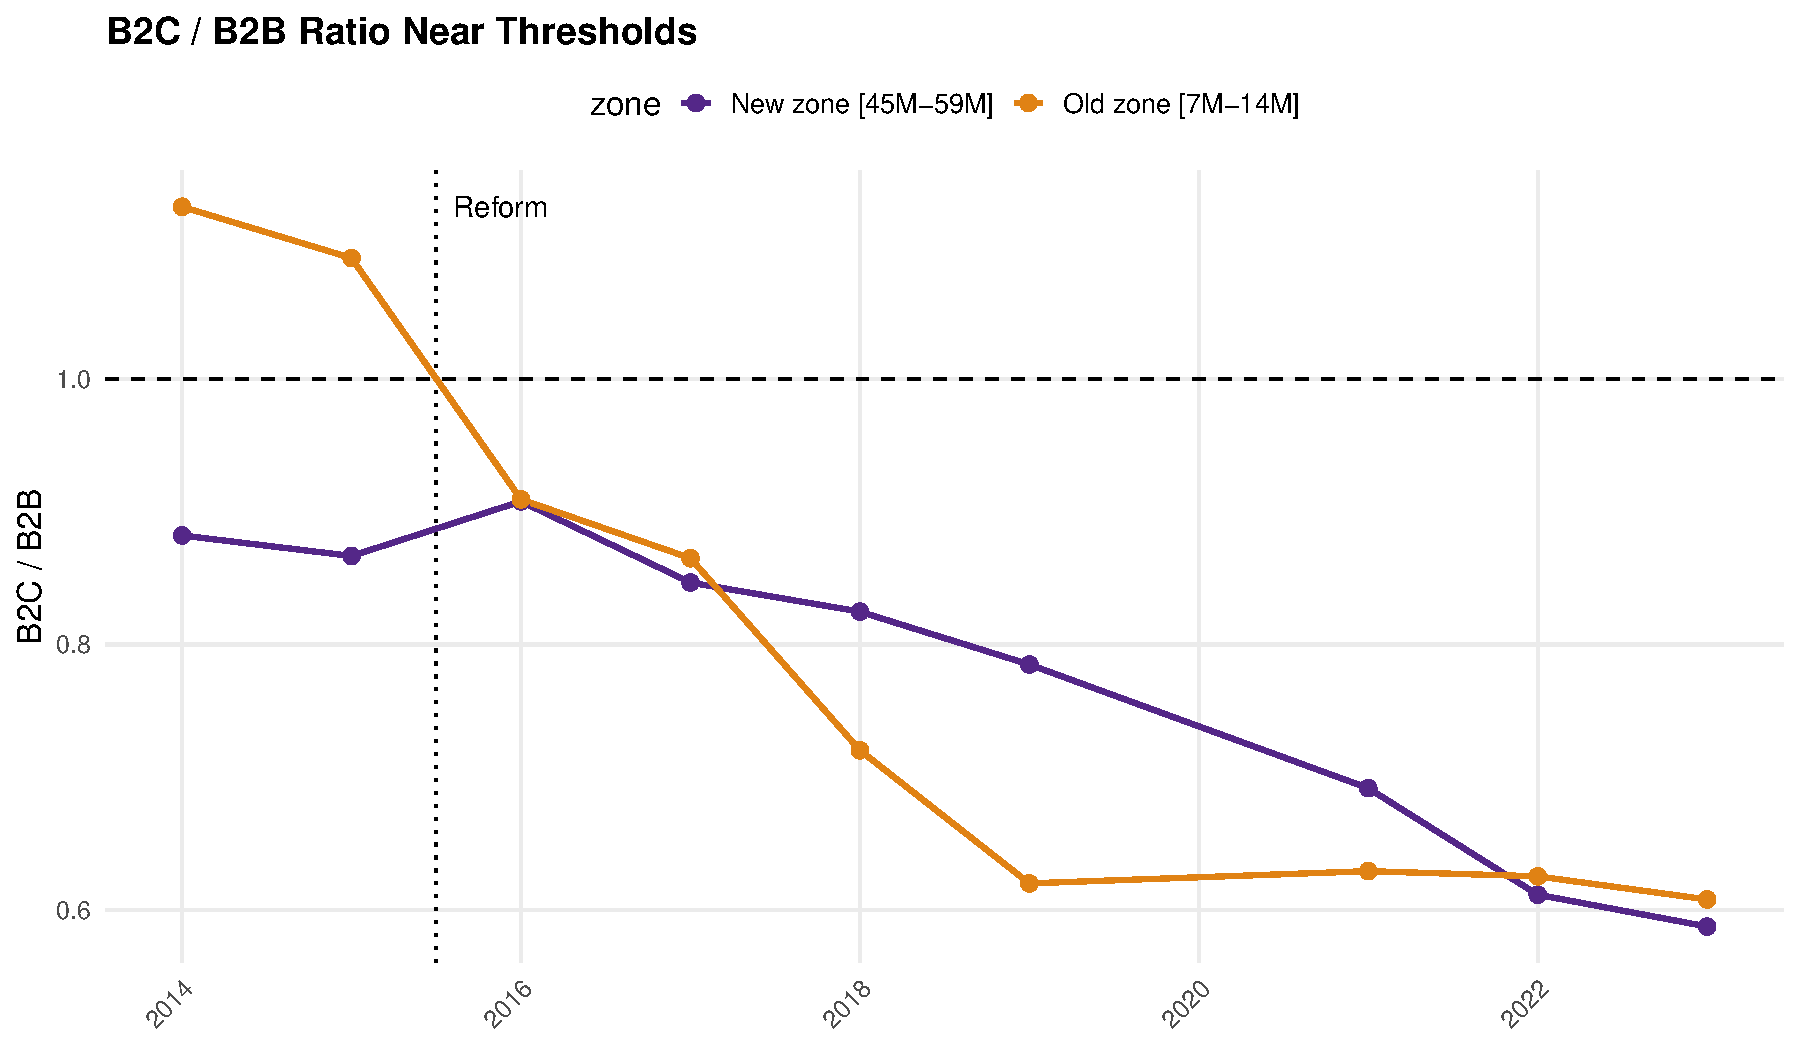
\includegraphics[width=0.9\linewidth]{Figures/fig_ratio.pdf}
\label{fig:ratio_threshold}

\small\textit{Source:} MTA CIT registry data.
\end{figure}

\vspace{1em}
% TABLE A.x Year-by-year threshold-zone composition
\begin{table}[H]
\centering
\caption{\textbf{Threshold-Zone Firm Counts and B2C/B2B Ratios by Year}}
\label{tab:app_zone_composition}
\begin{threeparttable}
\small
\begin{tabular*}{\linewidth}{l@{\extracolsep{\fill}}rrrrrr}
\toprule
& \multicolumn{3}{c}{\textit{Old zone $[7\text{M},15\text{M})$}}
& \multicolumn{3}{c}{\textit{New zone $[45\text{M},60\text{M})$}} \\
\cmidrule(lr){2-4}\cmidrule(lr){5-7}
Year & B2C & B2B & Ratio & B2C & B2B & Ratio \\
\midrule
2014 & 2,557 & 2,263 & 1.13 & 494 & 560 & 0.88 \\
2015 & 2,261 & 2,072 & 1.09 & 507 & 585 & 0.87 \\
2016 & 1,605 & 1,765 & 0.91 & 729 & 803 & 0.91 \\
2017 & 1,461 & 1,689 & 0.87 & 795 & 939 & 0.85 \\
2018 & 1,228 & 1,705 & 0.72 & 875 & 1,061 & 0.82 \\
2019 & 1,073 & 1,731 & 0.62 & 923 & 1,176 & 0.78 \\
2020 &   981 & 1,560 & 0.63 & 821 & 1,149 & 0.71 \\
2021 &   860 & 1,367 & 0.63 & 812 & 1,174 & 0.69 \\
2022 &   869 & 1,390 & 0.63 & 829 & 1,356 & 0.61 \\
2023 &   846 & 1,392 & 0.61 & 918 & 1,563 & 0.59 \\
\bottomrule
\end{tabular*}
\begin{tablenotes}[para,flushleft]\footnotesize
\item \textit{Source:} MTA CIT registry data. Counts are total active firms
  with lower bin edge in the stated revenue zone, summed across the two B2C
  sectors (retail, food service) and the two B2B sectors (wholesale,
  manufacturing). Ratio is B2C/B2B.
\end{tablenotes}
\end{threeparttable}
\end{table}

\clearpage
\begin{figure}[H]
\centering
\caption{\textbf{Pre-Reform Firm Distributions}}
\label{fig:app_dist_pre}

\begin{subfigure}{0.9\linewidth}
    \centering
    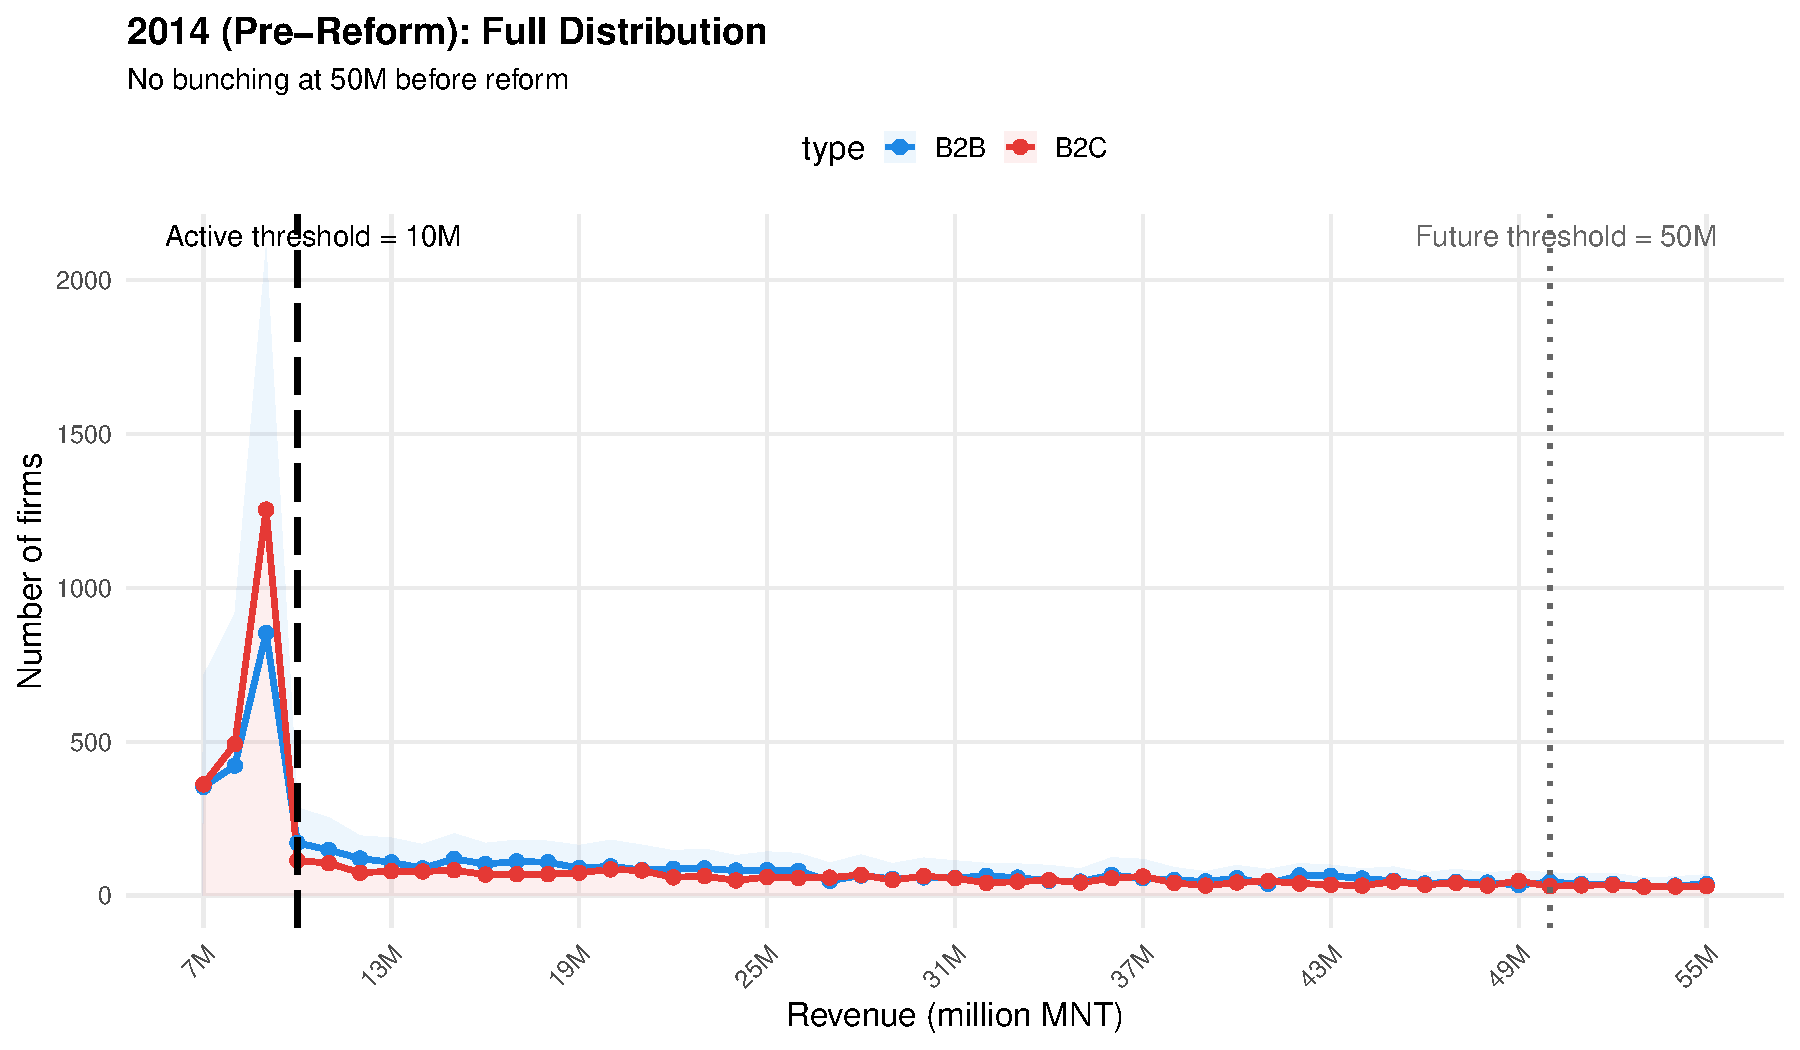
\includegraphics[width=\linewidth]{Figures/fig_2014_wide.pdf}
    \caption{2014: Full distribution (7M--55M)}
\end{subfigure}

\vspace{1em}

\begin{subfigure}{0.9\linewidth}
    \centering
    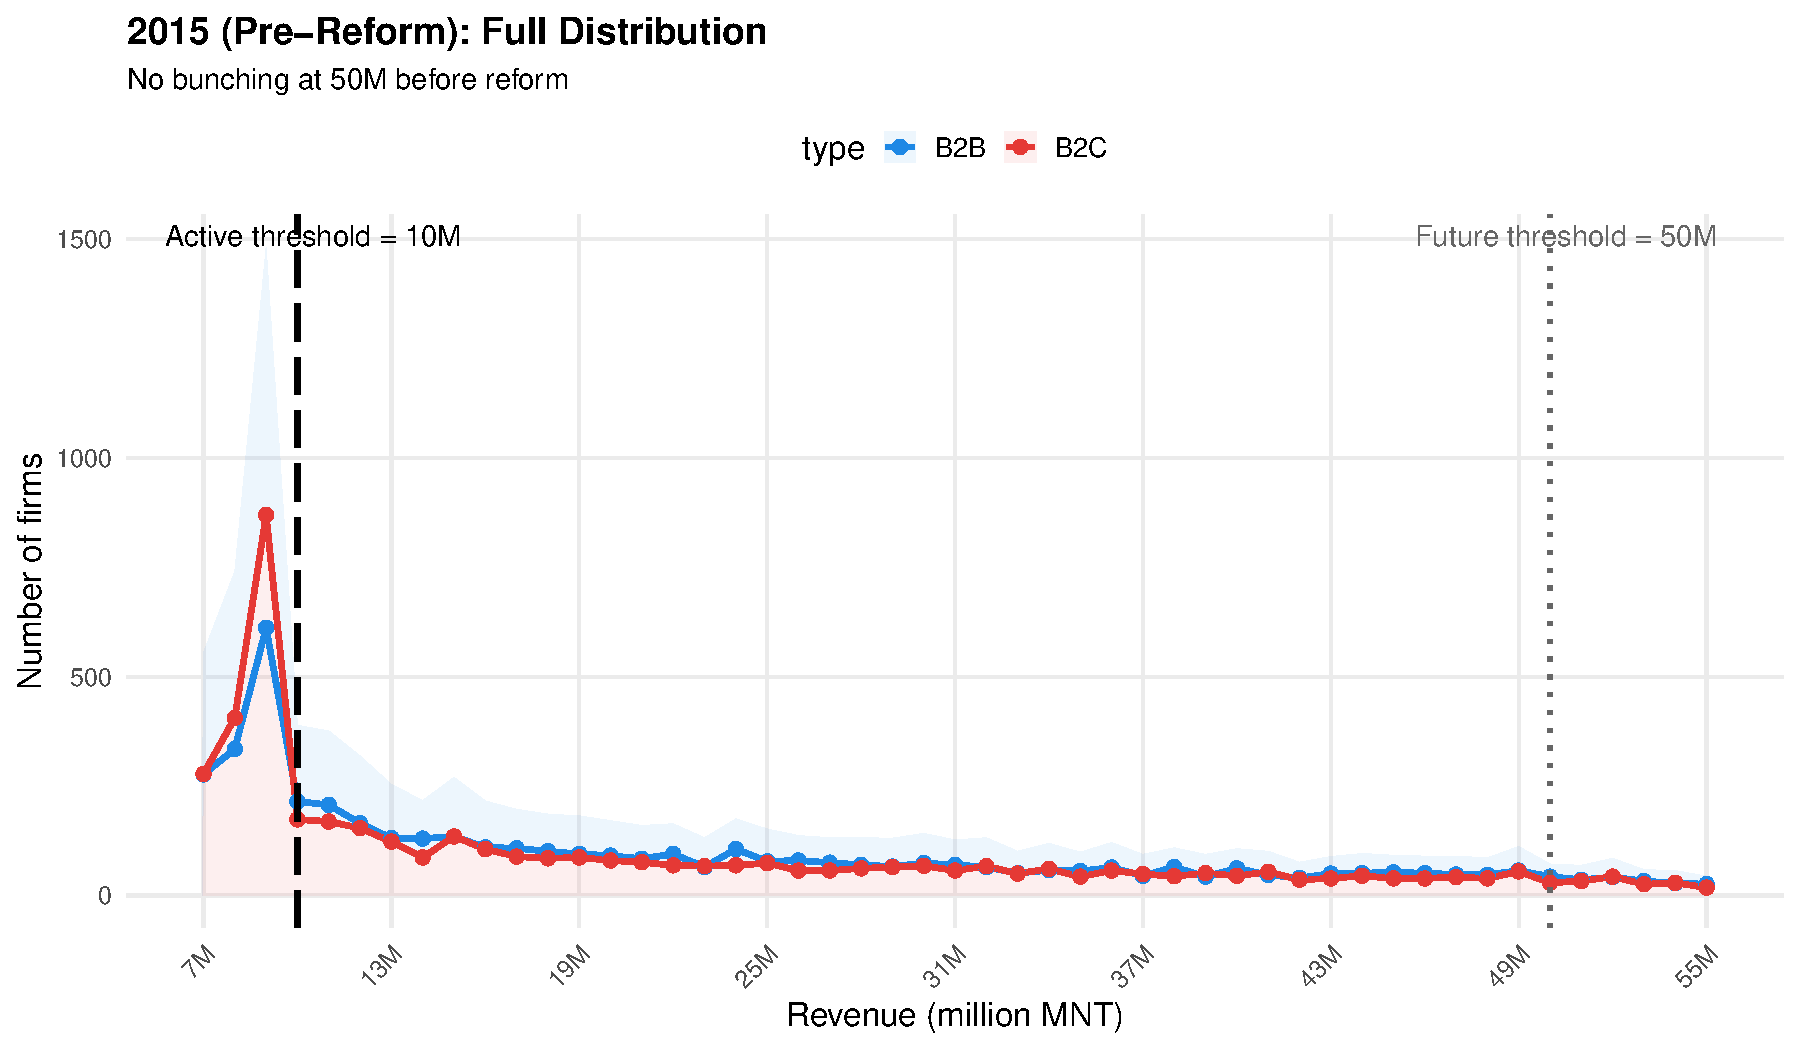
\includegraphics[width=\linewidth]{Figures/fig_2015_wide.pdf}
    \caption{2015: Full distribution (7M--55M)}
\end{subfigure}

\small\textit{Source:} MTA CIT registry data.
\end{figure}

\clearpage
\begin{figure}[H]
\centering
\caption{\textbf{Post-Reform Firm Distributions}}
\label{fig:app_dist_post}

\begin{subfigure}{0.9\linewidth}
    \centering
    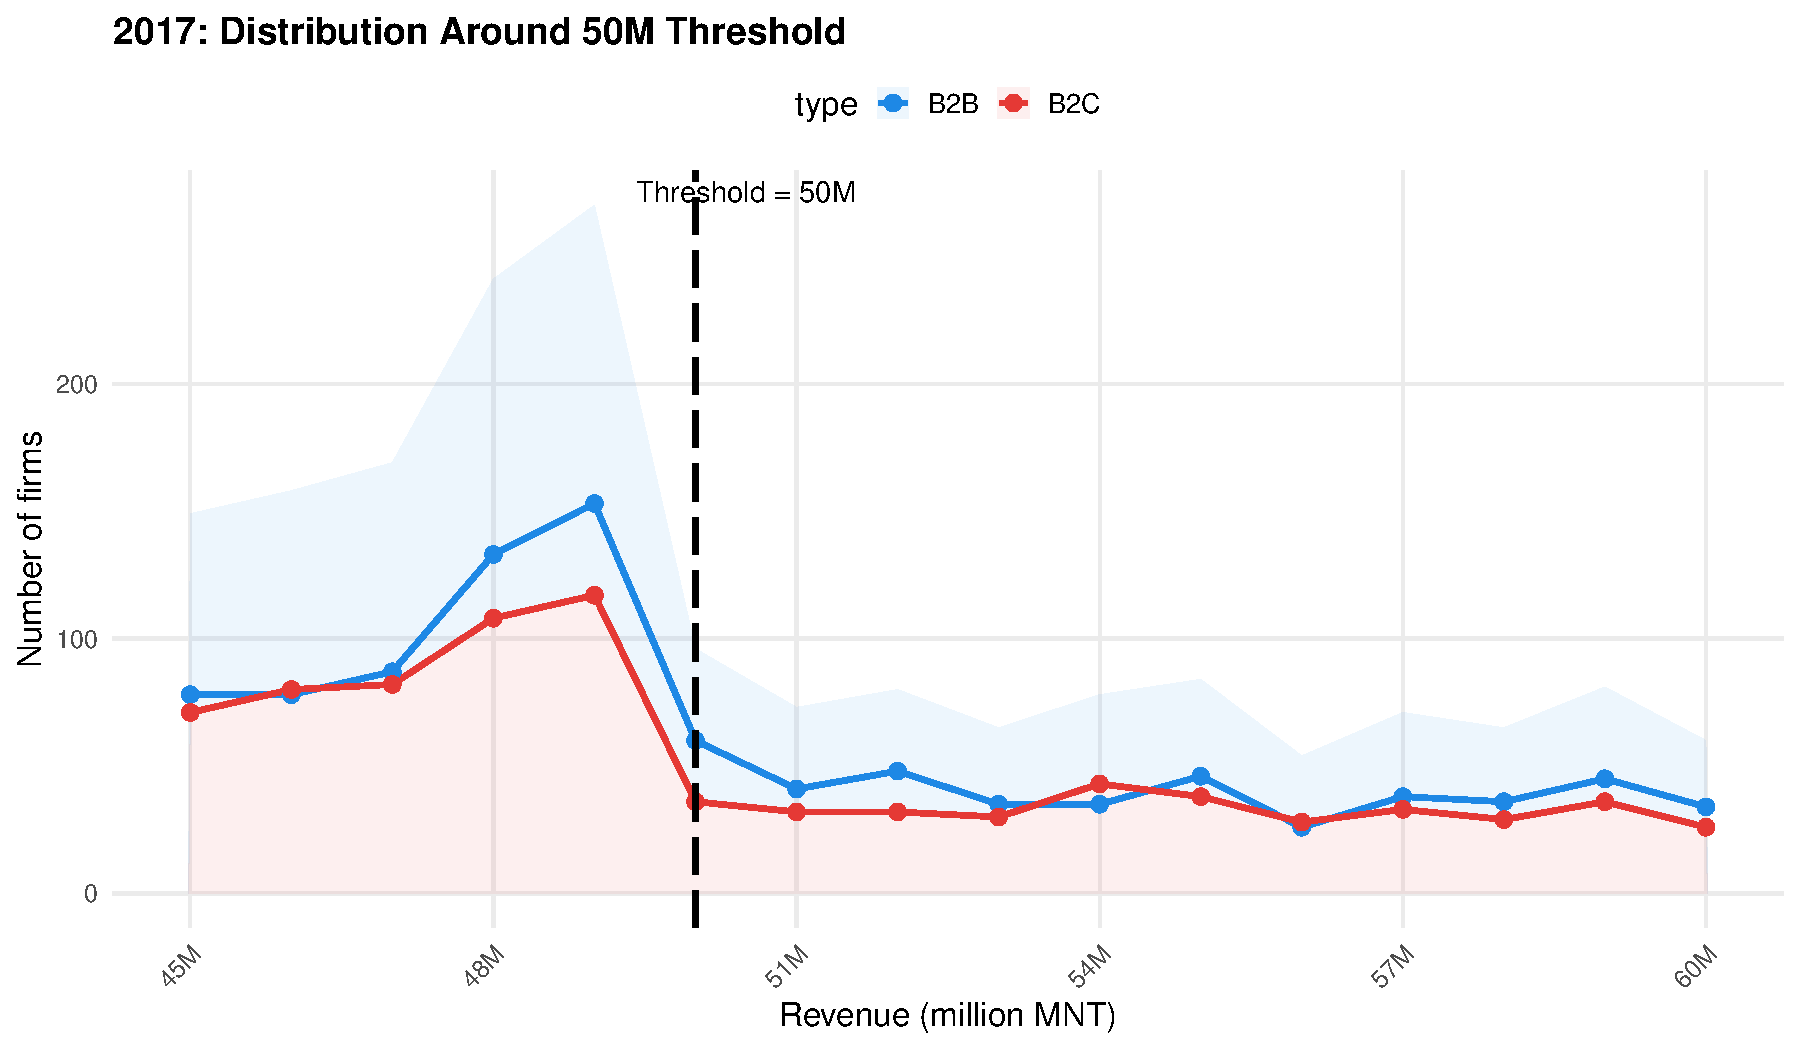
\includegraphics[width=\linewidth]{Figures/fig_2017.pdf}
    \caption{2017: Around 50M threshold}
\end{subfigure}

\vspace{1em}

\begin{subfigure}{0.9\linewidth}
    \centering
    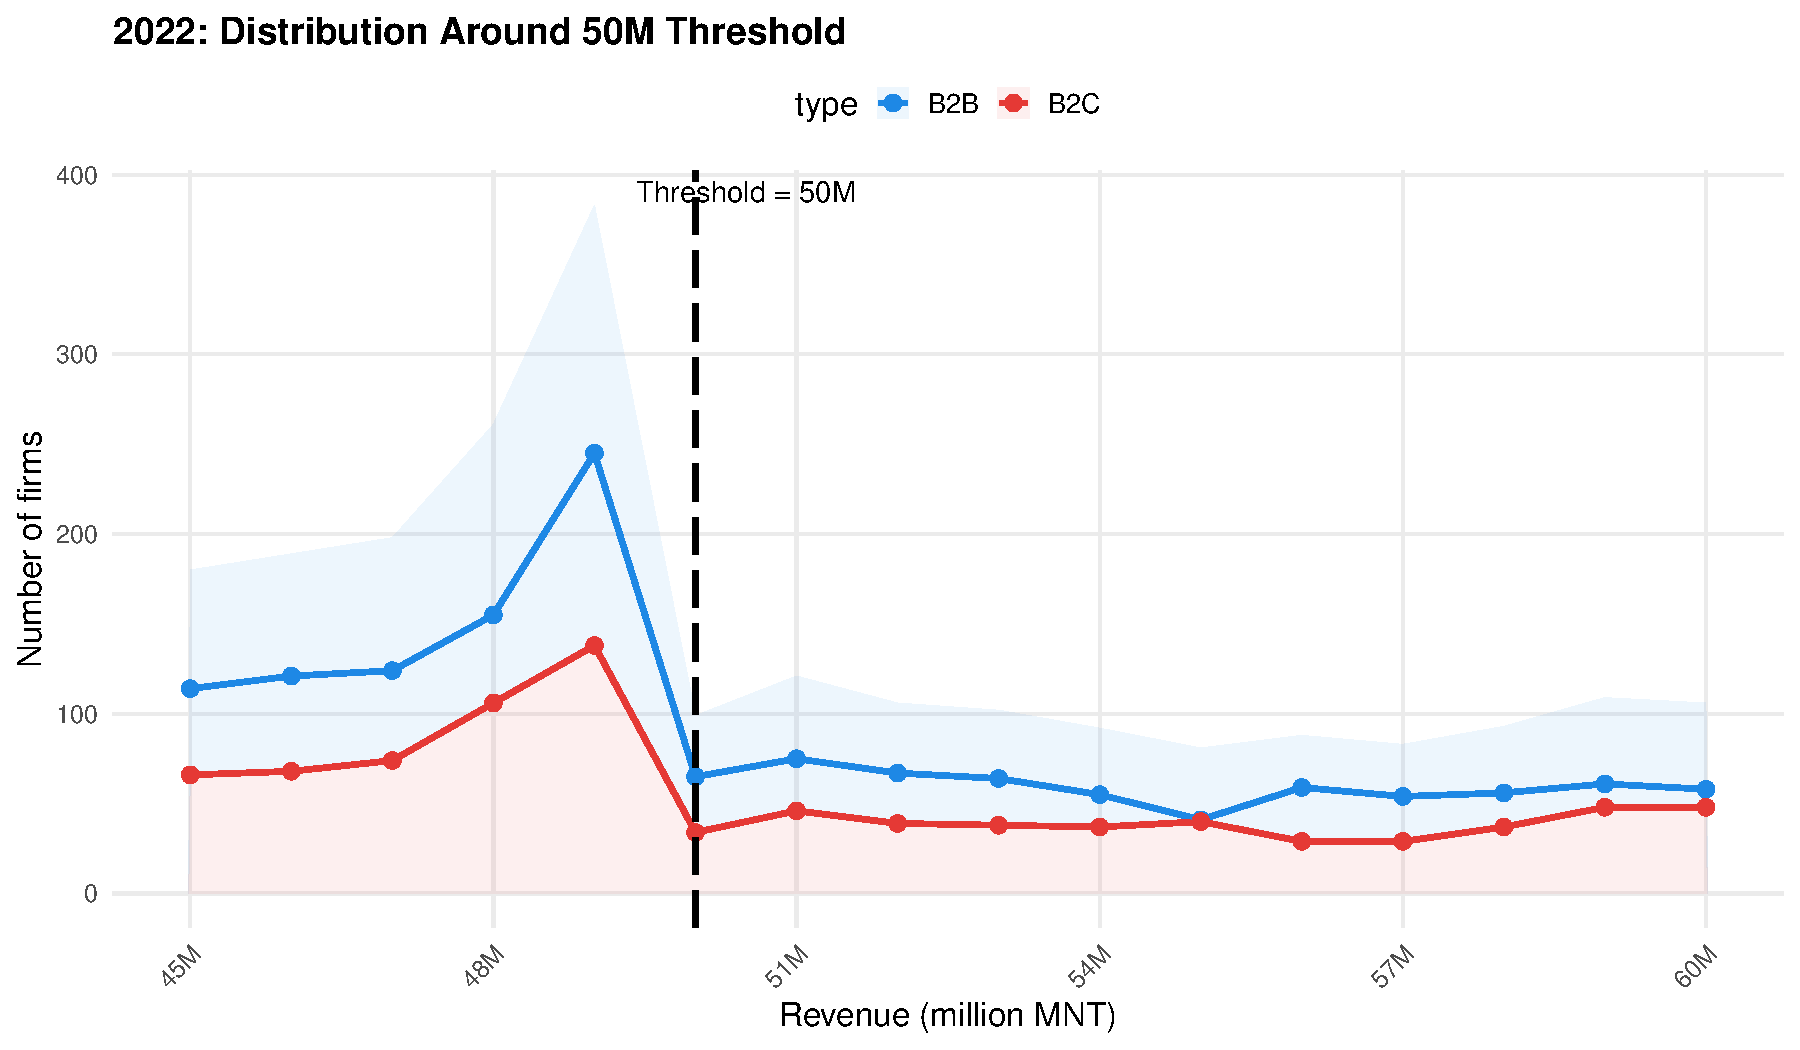
\includegraphics[width=\linewidth]{Figures/fig_2022.pdf}
    \caption{2022: Around 50M threshold}
\end{subfigure}

\small\textit{Source:} MTA CIT registry data.
\end{figure}




%TABLE A.2 Normalised Bunching Estimates
\renewcommand{\arraystretch}{0.9}
\begin{table}[H]
\centering
\caption{\textbf{Normalised Bunching Estimates $\hat{b}_{st}$ by Sector and Year (Main Sample)}}
\label{tab:app_bunching_main}
\begin{threeparttable}
\setlength{\tabcolsep}{0pt}
\small
\begin{tabular*}{\linewidth}{l@{\extracolsep{\fill}}ccccccccc}
\toprule
Sector & 2014 & 2015 & 2016 & 2017 & 2018 & 2019 & 2021 & 2022 & 2023 \\
\midrule
\multicolumn{10}{l}{\textit{B2C Treatment Group}} \\[2pt]
\quad Retail           & 4.368\dag & 4.050\dag & 2.089 & 1.755 & 2.417 & 2.220 & 1.487 & 1.919 & 1.703 \\
               & (0.263) & (0.189) & (0.169) & (0.167) & (0.210) & (0.183) & (0.154) & (0.167) & (0.150) \\[4pt]
\quad Food Service     & 3.945\dag & 2.411\dag & 2.282 & 1.579 & 1.257 & 2.565 & 0.564 & 4.099 & 1.585 \\
               & (0.430) & (0.310) & (0.575) & (0.415) & (0.284) & (0.469) & (0.409) & (1.633) & (0.455) \\[4pt]
\multicolumn{10}{l}{\textit{B2B Control Group}} \\[2pt]
\quad Wholesale        & 2.301 & 2.033\dag & 1.989 & 2.088 & 2.017 & 1.904 & 1.700 & 2.048 & 3.006 \\
               & (0.150) & (0.121) & (0.177) & (0.160) & (0.183) & (0.141) & (0.159) & (0.181) & (0.178) \\[4pt]
\quad Manufacturing    & 3.018\dag & 1.655\dag & 0.952 & 2.592\dag & 3.665\dag & 2.096 & 0.959 & 2.063 & 2.133 \\
               & (0.215) & (0.148) & (0.259) & (0.462) & (1.009) & (0.284) & (0.226) & (0.241) & (0.273) \\[4pt]
\midrule
\textit{B2C Mean} & 4.156 & 3.230 & 2.185 & 1.667 & 1.837 & 2.392 & 1.026 & 3.009 & 1.644 \\
\textit{B2B Mean} & 2.660 & 1.844 & 1.471 & 2.340 & 2.841 & 2.000 & 1.330 & 2.056 & 2.570 \\
\midrule
\textit{Gap (B2C $-$ B2B)} & $+$1.497 & $+$1.386 & $+$0.715 & $-$0.673 & $-$1.004 & $+$0.393 & $-$0.304 & $+$0.953 & $-$0.926 \\
\bottomrule
\end{tabular*}
\begin{tablenotes}[para,flushleft]\footnotesize
\item \textit{Notes:} $\hat{b}_{st}$ from a degree 5 pre-reform, degree 7 post-reform counterfactual. Exclusion window $[z^*_t - 2M,\, z^*_t + 30M)$ post-reform, $[z^*_t - 2M,\, z^*_t + 10M)$ pre-reform. Bootstrap standard errors (500 replications) in parentheses.
Negative values indicate deficits relative to the counterfactual.
2020 excluded from this table.
\item[$\dag$] Missing mass did not reach bunching mass within the cap
Capped cells.
\textit{Source:} Author's calculations based on MTA CIT registry data.
\end{tablenotes}
\end{threeparttable}
\end{table}

%TABLE A.3 Bunching Estimates COVID
\begin{table}[H]
\centering
\caption{\textbf{Bunching Estimates in Pandemic Years (2020 and 2021)}}
\label{tab:app_covid}
\begin{threeparttable}
\setlength{\tabcolsep}{10pt}
\small
\begin{tabular}{lrrrrrr}
\toprule
 & \multicolumn{3}{c}{2020} & \multicolumn{3}{c}{2021} \\
\cmidrule(lr){2-4}\cmidrule(lr){5-7}
Sector & $\hat{b}$ & SE & 95\% CI & $\hat{b}$ & SE & 95\% CI \\
\midrule
Retail (B2C)         & 1.581 & 0.181 & [1.235,\; 1.957] & 1.487 & 0.154 & [1.197,\; 1.790] \\
Food Service (B2C)   & 1.301 & 0.382 & [0.693,\; 2.222] & 0.564 & 0.409 & [-0.078,\; 1.490] \\
Wholesale (B2B)      & 1.119 & 0.147 & [0.855,\; 1.418] & 1.700 & 0.159 & [1.420,\; 2.047] \\
Manufacturing (B2B)  & 2.635 & 0.635 & [1.705,\; 4.081] & 0.959 & 0.226 & [0.593,\; 1.500] \\
\midrule
\textit{B2C mean} & 1.441 & & & 1.026 & & \\
\textit{B2B mean} & 1.877 & & & 1.330 & & \\
\textit{Gap (B2C $-$ B2B)} & $-$0.436 & & & $-$0.304 & & \\
\bottomrule
\end{tabular}
\begin{tablenotes}[para,flushleft]\footnotesize
\item \textit{Notes:} 2020 observations are excluded from the Main and
Robustness A samples but retained in the Full sample.
2021 observations are included in Main but excluded from Robustness A.
Bootstrap standard errors based on 500 replications.
\textit{Source:} Author's calculations based on MTA CIT registry data.
\end{tablenotes}
\end{threeparttable}
\end{table}

% ── APPENDIX FIGURE A.2 ──
\begin{figure}[H]
    \centering
    \caption{\textbf{Observed Distribution and Polynomial Counterfactual: 2015 (Pre-Reform)}}
    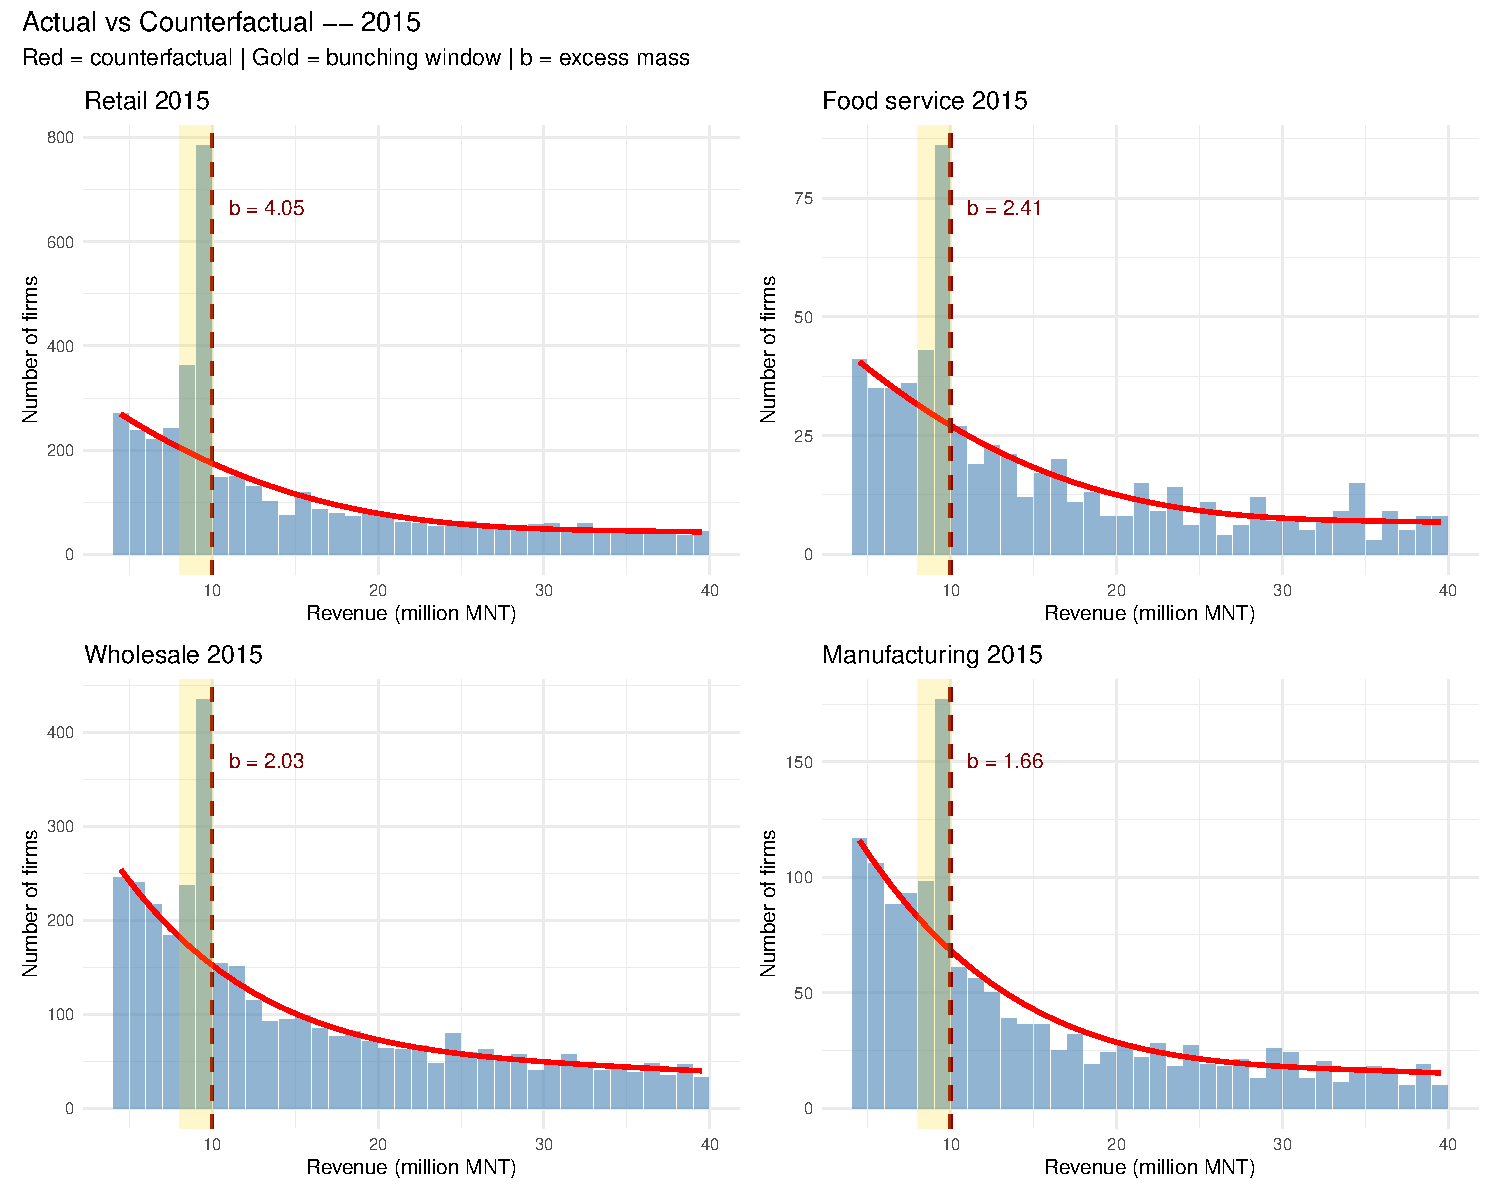
\includegraphics[width=\textwidth]{Figures/fig5_counterfactual_2015.pdf}
    \label{fig:app_cf_2015}

    \footnotesize\textit{Notes:} Observed firm counts by revenue bin (bars) are
    plotted alongside the fitted polynomial counterfactual (red line).
    The shaded region denotes the exclusion window ($R_t$) around the VAT
    registration threshold. The active threshold is $z^* = 10$M MNT.
    Excess mass below the threshold relative to the counterfactual
    identifies bunching behaviour. \textit{Source:} Author’s calculations based on MTA CIT registry data.
\end{figure}

\begin{figure}[H]
    \centering
    \caption{\textbf{Observed Distribution and Polynomial Counterfactual: 2022 (Post-Reform)}}
    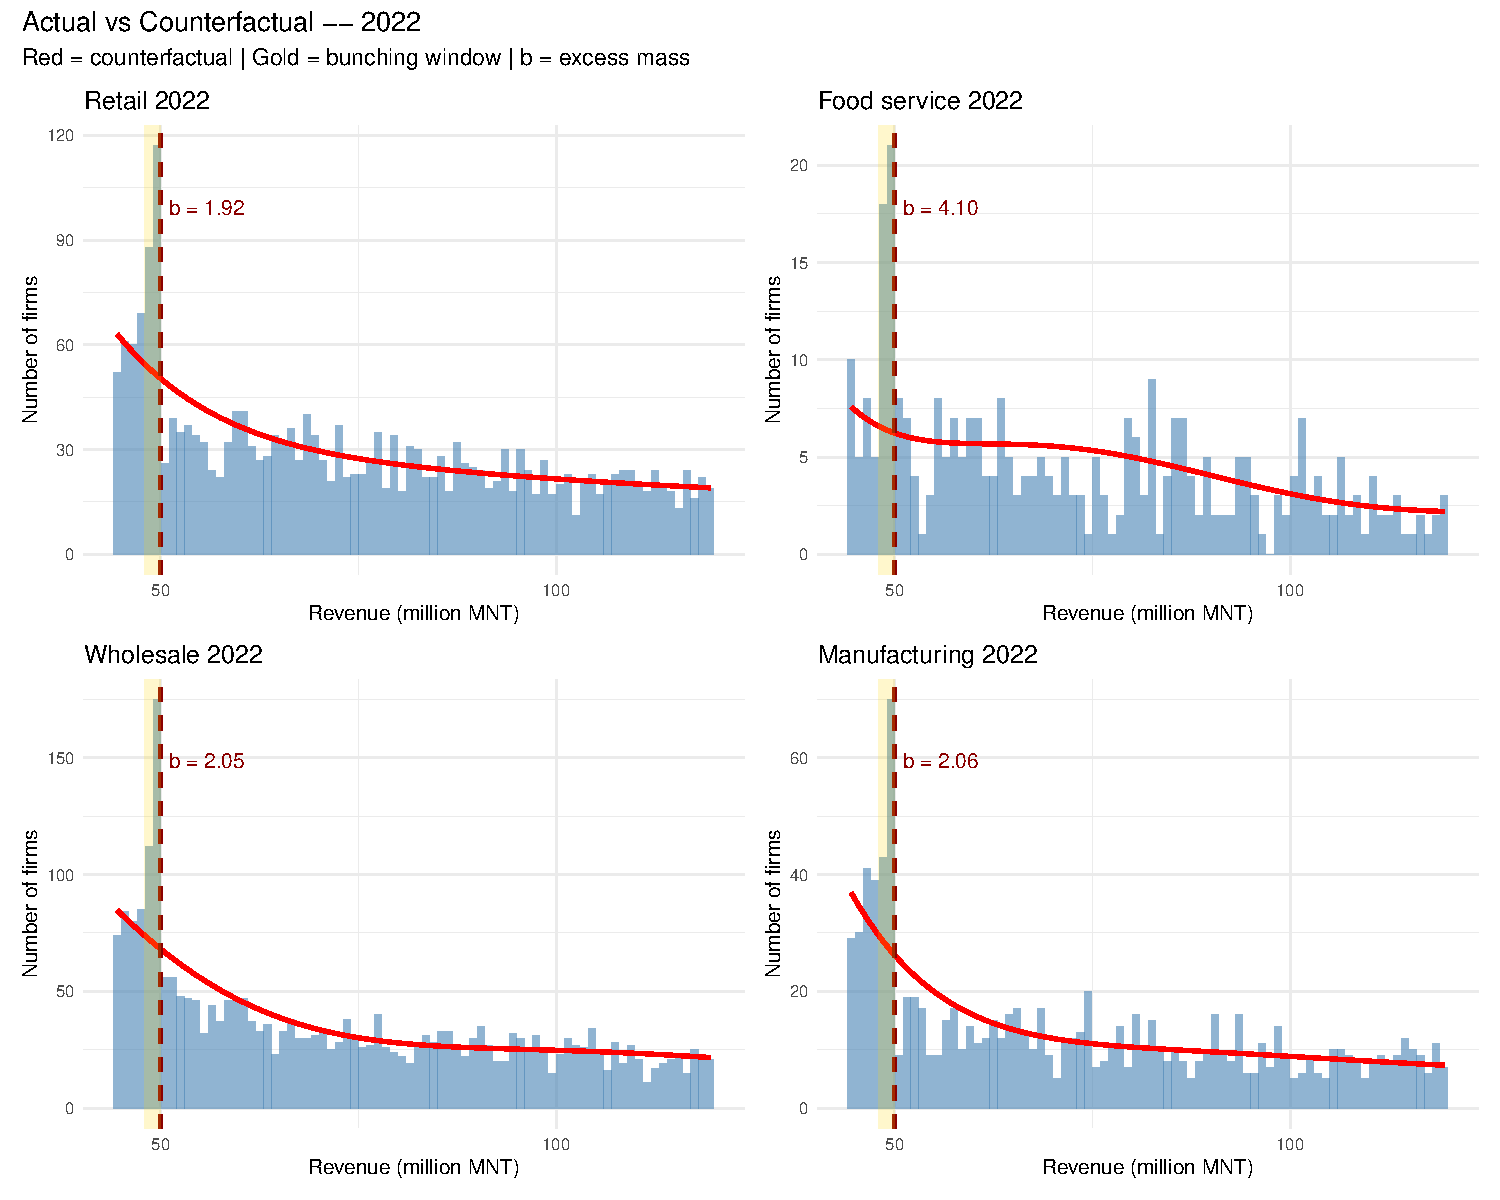
\includegraphics[width=\textwidth]{Figures/fig5_counterfactual_2022.pdf}
    \label{fig:app_cf_2022}

    \footnotesize\textit{Notes:} Observed firm counts by revenue bin (bars) are
    plotted alongside the fitted polynomial counterfactual (red line).
    The shaded region denotes the exclusion window ($R_t$) around the VAT
    registration threshold. The active threshold is $z^* = 50$M MNT.
    Relative to 2015, reduced excess mass below the threshold is consistent
    with improved enforcement following the introduction of ebarimt. \textit{Source:} Author’s calculations based on MTA CIT registry data.
\end{figure}


% ────────────────────────────────────────────
% APPENDIX B SECTION
% ────────────────────────────────────────────
\clearpage
\section{Robustness and Sensitivity Checks}
\label{sec:appendix_robustness_sensitivity}

This appendix reports the robustness checks referenced in Chapter~\ref{ch:results}: the DiD re-estimated with manufacturing as the sole control, and the sensitivity of the bunching estimates to the polynomial degree (Table~\ref{tab:app_robust_polynomial}) and the bunching-window width (Table~\ref{tab:app_excl_lo}).

\vspace{1em}
\noindent\textbf{Manufacturing-only control group.}
Table~\ref{tab:app_robust_mfg} re-estimates the DiD with manufacturing as the only control. Dropping wholesale removes the control sector most exposed to upstream spillovers (Section~\ref{sec:event}), leaving a comparison group with no consumer-facing sales. The estimate stays negative and close to the four-sector benchmark across all three samples ($\hat{\beta}$ between $-1.457$ and $-1.593$, against $-1.562$ in the main specification).

% ── TABLE B.1: MANUFACTURING-ONLY DIID SENSITIVITIES ──
\begin{table}[H]
\centering
\caption{\textbf{Difference-in-Differences Sensitivities: Manufacturing-Only Control Group}}
\label{tab:app_robust_mfg}
\begin{threeparttable}
\setlength{\tabcolsep}{12pt}
\small
\begin{tabular}{lccc}
\toprule
 & (1) Main & (2) Robustness A & (3) Full Sample \\
 & (2020 excl.) & (2020+21 excl.) & (all years) \\
\midrule
$\hat{\beta}$: $\text{Post} \times \text{Treated}$
  & $-1.457^{**}$ & $-1.484^{**}$ & $-1.593^{***}$ \\
  & $(0.563)$ & $(0.627)$ & $(0.538)$ \\
\midrule
Sector + Year FE & Yes & Yes & Yes \\
$N$ (cells) & 27 & 24 & 30 \\
\bottomrule
\end{tabular}
\begin{tablenotes}[para,flushleft]\footnotesize
\item \textit{Notes:} HC2 heteroskedasticity-robust standard errors in
parentheses (wild cluster bootstrap not applied here as $G = 3$); with three clusters HC2 inference is anti-conservative, so the markers are indicative and formal inference rests on the four-cluster bootstrap in Table~\ref{tab:did}.
$^{*}p < 0.10$, $^{**}p < 0.05$, $^{***}p < 0.01$.
Treatment group: B2C (retail, food services).
Control group: manufacturing only (wholesale excluded).
\textit{Source:} Author's calculations based on MTA CIT registry data.
\end{tablenotes}
\end{threeparttable}
\end{table}

\vspace{1em}
\noindent\textbf{Sensitivity to polynomial degree.}
Table~\ref{tab:app_robust_polynomial} varies the counterfactual polynomial from degree 5 to degree 8, holding all else fixed. The estimates are stable across degrees 5 to 7 for nearly every cell. The 2022 food service reading ($\hat{b} = 4.099$) is an outlier against the sector's declining trend, resting on a sparse near-threshold distribution: it holds across degrees 5 to 7 but overfits to 6.532 at degree 8, which marks the cell as fragile (Appendix Table~\ref{tab:app_robust_polynomial}). The baseline specification (degree 5 pre-reform, degree 7 post-reform) balances flexibility against this risk.

% ── TABLE B.2: POLYNOMIAL DEGREE SENSITIVITIES ──
\begin{table}[H]
\centering
\caption{\textbf{Sensitivity of Bunching Estimates to Polynomial Degree: Selected Sector-Year Cells}}
\label{tab:app_robust_polynomial}
\begin{threeparttable}
\setlength{\tabcolsep}{12pt}
\small
\begin{tabular}{lcccc}
\toprule
 & Degree 5 & Degree 6 & Degree 7 & Degree 8 \\
Sector-Year & & & (Baseline, $p=7$) & \\
\midrule
\multicolumn{5}{l}{\textit{Panel A: Pre-Reform (2015, $z^* = 10M$ MNT)}} \\[2pt]
\quad Retail 2015          & 4.050 & 3.790 & 3.820 & 3.652 \\
\quad Food service 2015    & 2.411 & 2.180 & 2.161 & 1.994 \\
\quad Wholesale 2015       & 2.033 & 2.069 & 2.120 & 2.341 \\
\quad Manufacturing 2015   & 1.655 & 1.665 & 1.676 & 1.575 \\
[6pt]
\multicolumn{5}{l}{\textit{Panel B: Post-Reform (2022, $z^* = 50M$ MNT)}} \\[2pt]
\quad Retail 2022          & 1.881 & 1.890 & 1.919 & 1.839 \\
\quad Food service 2022    & 3.678 & 3.618 & 4.099 & 6.532 \\
\bottomrule
\end{tabular}
\begin{tablenotes}[para,flushleft]\footnotesize
\item \textit{Notes:} Exclusion window $[z^*_t - 2M,\, z^*_t + 30M)$ post-reform, $[z^*_t - 2M,\, z^*_t + 10M)$ pre-reform.
Degree 7 is the baseline specification.
\textit{Source:} Author's calculations based on MTA CIT registry data.
\end{tablenotes}
\end{threeparttable}
\end{table}

\vspace{1em}
\noindent\textbf{Sensitivity to window width.}
Table~\ref{tab:app_excl_lo} varies the bunching window below the threshold. The baseline 2-bin window ($[z^*_t - 2\text{M},\, z^*_t)$) gives $\hat{\beta} = -1.562$; widening to 3 bins keeps the negative sign ($\hat{\beta} = -0.974$) and an 80\% post-reform narrowing. At 4 bins and beyond the window reaches into the rising pre-notch slope of the small-firm density, the pre-reform gap turns sharply negative, and the estimates break down. A window of $\delta \in \{2,3\}$ is therefore the admissible range, as Section~\ref{sec:estimation_method} notes.

% TABLE B.3 Sensitivity of DiD Estimates excl_lo
\begin{table}[H]
\centering
\caption{\textbf{Sensitivity of DiD Estimate to Bunching Window Width ($\texttt{excl\_lo}$ Sweep)}}
\label{tab:app_excl_lo}
\begin{threeparttable}
\setlength{\tabcolsep}{4pt} % Reduced from 6pt to save horizontal space
\small
\begin{tabular}{lcccccccc}
\toprule
% Simplified header (explanation is already in footnote 'a')
$\delta$\tnote{a} & B2C pre & B2C post & B2B pre & B2B post
  & Gap pre & Gap post & DiD & \% narrow \\
\midrule
$2\dag$ & 3.693 & 1.966 & 2.252 & 2.087 & $+$1.441 & $-$0.121 & $-1.562$ & 108\% \\
$3$ & 4.703 & 2.542 & 3.481 & 2.294 & $+$1.222 & $+$0.248 & $-0.974$ & 80\% \\
$4$ & 17.078 & 2.569 & 97.370 & 2.512 & $-$80.291 & $+$0.056 & $80.348$ & 100\% \\
$5$ & 26.216 & 2.856 & 105.689 & 3.203 & $-$79.473 & $-$0.347 & $79.126$ & 100\% \\
\bottomrule
\end{tabular}
\begin{tablenotes}[para,flushleft]\footnotesize
\item \textit{Notes:} Each row re-estimates all sector-year cells with a bunching window of $[z^*_t - \delta\text{M},\, z^*_t)$. DiD = $(\Delta\bar{b}_{B2C}) - (\Delta\bar{b}_{B2B})$, main sample (2020 excluded). \% narrowing $= (\text{gap}_{\text{pre}} - \text{gap}_{\text{post}}) / \text{gap}_{\text{pre}} \times 100$.
\item[$\dag$] Locked specification ($\delta = 2$).
\item[a] Window width in 1M MNT bins below the threshold.
DiD sign is stable at $\delta \in \{2,3\}$; larger windows
extend into the ascending pre-notch slope and are not reported as admissible.
\textit{Source:} Author's calculations based on MTA CIT registry data.
\end{tablenotes}
\end{threeparttable}
\end{table}


\printbibliography
\end{document}
